%\documentclass[preprint,12pt]{elsarticle}

%% Use the options 1p,twocolumn; 3p; 3p,twocolumn; 5p; or 5p,twocolumn
%% for a journal layout:
%\documentclass[final,1p,times]{elsarticle}
%% \documentclass[final,1p,times,twocolumn]{elsarticle}
%% \documentclass[final,3p,times]{elsarticle}
%\documentclass[final,3p,times,twocolumn]{elsarticle}
%\documentclass[preprint,5p,times]{elsarticle}
\documentclass[final,5p,times,twocolumn]{elsarticle}
\biboptions{sort&compress}

\usepackage{amssymb}
\usepackage{amsmath}
\usepackage{multirow, subfig, tabularx, booktabs}
\usepackage{xcolor}
\usepackage[flushleft]{threeparttable}
\usepackage{algorithm}
\usepackage{algpseudocode}
\usepackage{caption}
\usepackage{enumitem}
\usepackage{multicol}
%\usepackage[ruled,vlined]{algorithm2e}

%\usepackage[ruled,vlined]{algorithm2e}
%\usepackage{algpseudocode}
%% \begin{linenumbers}, end it with \end{linenumbers}. Or switch it on
%% for the whole article with \linenumbers.
\usepackage{lineno}
\usepackage{graphicx}
\usepackage{array}
\usepackage{float}
\usepackage{textcomp}
\usepackage{mathrsfs}

\newcommand{\added}[1]{#1}

\journal{Remote Sensing Applications: Society and Environment}

\begin{document}
%\linenumbers

\begin{frontmatter}

%\title{Rice Variety Discrimination Based on NIR Hyperspectral Imaging: Impact of Variable Selection Methods}

\title{Rice variety discrimination by NIR hyperspectral imaging: validation design, accuracy metric and variable selection}

\author[1]{Himer Avila-George}
\author[2]{Nicole Briceño}
\ead{2019203003@unf.edu.pe}
\author[2]{Cecilia Risco}
\ead{crisco@unf.edu.pe}
\author[3]{Tony Chuquizuta}
\ead{tchuquizuta@unach.edu.pe}
\author[4,5]{Aldo F. Combariza}
\ead{aldo.combariza@unisucre.edu.co}
\author[6]{Wilson Castro\corref{cor1}}
\ead{wcastro@unf.edu.pe}
\cortext[cor1]{Corresponding author}

%% Author affiliation
\affiliation[1]{organization={Centro de Investigación en Procesamiento Digital de Señales, Universidad de Guadalajara}, city={Ameca}, state={Jalisco}, country={México}}

\affiliation[2]{organization={Facultad de Ciencias Económicas y Ambientales, Universidad Nacional de Frontera}, addressline={Av. San Hilarión N° 101}, city={Sullana}, postcode={20100}, state={Piura}, country={Perú}}

\affiliation[3]{organization={Grupo de Investigación en Tecnologías Emergentes Fotónicas (GITEF), Instituto de Investigación del Mejoramiento Productivo, Universidad Nacional Autónoma de Chota}, city={Chota}, postcode={06120}, state={Cajamarca}, country={Perú}}

\affiliation[4]{organization={Departamento de Biología y Química, Facultad de Educación y Ciencias, Universidad de Sucre}, city={Sincelejo}, country={Colombia}}

\affiliation[5]{organization={Programa de Doctorado en Ciencias Físicas, SUE Caribe}, country={Colombia}}

\affiliation[6]{organization={Facultad de Ingeniería de Industrias Alimentarias y Biotecnología, Universidad Nacional de Frontera}, addressline={Av. San Hilarión N° 101}, city={Sullana}, postcode={20100}, state={Piura}, country={Perú}}

%% Abstract
\begin{abstract}
Near-infrared hyperspectral imaging (NIR-HSI) is widely proposed for authenticating rice varieties, and published accuracies often exceed 95\%. We examine how far such figures depend on the validation design, the metric and band selection. Mean spectra of 500 grains of each of twelve Peruvian varieties (Resonon Pika NIR-640, 263 bands, 999--1649~nm) were classified with a linear support vector machine on standardized bands (SVM), a linear SVM on unstandardized bands (L-SVM), linear discriminant analysis (LDA) and a neural network (ANN), on the full spectrum and on bands selected by neighborhood component analysis (FSCNCA), sequential forward selection (SFS) and covering-array feature selection (CAFS). Classifiers were validated by five-fold cross-validation with grains assigned at random or with whole images held out, and each selected band subset was compared against randomly drawn subsets of the same size. The mean per-class one-vs-rest accuracy equals $1-2e/K$ for any confusion matrix ($e$ the overall error rate, $K$ the number of classes) and cannot fall below 83.3\% for twelve classes; 99.53\% for the SVM corresponds to 97.2\% overall. With grains divided at random, the SVM and the ANN reached 97\% overall accuracy and LDA and the L-SVM 90\%; with whole images held out, 88\%, 88\%, 87\% and 84\%. With selection fitted on training data only, SFS beat random subsets only with 5--10 bands (by about 4--9 points), and FSCNCA and CAFS never did. Reporting overall accuracy, validating on images not used for training and benchmarking band selection against random subsets would make accuracies comparable between studies.
\end{abstract}

%% Keywords
\begin{keyword}
Food fraud detection \sep  Grouped validation \sep  Rice authentication \sep NIR hyperspectral imaging \sep Machine learning \sep Cross-validation \sep Variable selection
\end{keyword}

\end{frontmatter}


% ================================================================================================
%% INTRODUCTION
% ================================================================================================

\section{Introduction}\label{sec1}

% 1) Reice global importance nutritional and economic; compositional variation due to variety 
Rice (\textit{Oryza sativa} L.) is the staple food of more than half the world's population, providing approximately 20\% of the daily caloric intake of more than 3.5 billion people \citep{subbuthavamurugan2023}; it is of particular relevance in Asian countries such as China, India, Thailand, and Indonesia \citep{Muthayya2014}. 
In China, annual rice production represents approximately 28\% of global production, while in Vietnam, rice constitutes a fundamental pillar of the national economy and food security \citep{Giang2020b, Tong2021}. 
Rice composition varies significantly between varieties, with differences in starch structure (amylose and amylopectin content), protein content, lipid content, and volatile compounds that directly influence cooking behavior, texture, aroma, and overall sensory quality \citep{Sampaio2019,Xie2024}. 
These compositional differences, largely determined by genetic background and growing conditions, underlie the price premiums that some varieties command.

% 2) Adulteration in rice grains using economic varieties 
The growing consumer demand for high-quality rice has generated a market in which premium varieties such as Thai jasmine rice, basmati, Wuyou No.4, and Wuchang aromatic rice command substantially higher prices than conventional varieties \citep{Teye2022, Tong2021, Sun2025, Zaresani2024}. 
This economic disparity has incentivized fraudulent practices involving the adulteration of premium varieties with lower-quality varieties or the falsification of geographical origin, a phenomenon that has reached alarming proportions \citep{Teye2022, SliwinskaBartel2021}. 
In the Chinese market, the volume of rice commercialized under the name ``Wuchang Daohuaxiang'' exceeds the actual production by more than tenfold, evidencing the magnitude of the problem \citep{Sun2025, Li2025}. 
This situation not only economically harms consumers and legitimate producers, but also compromises trust in quality control systems and food safety \citep{Shi2025, Rahmani2022, SliwinskaBartel2021}. 
The detection of adulteration in rice grains using economically valuable varieties has therefore become a priority for food regulatory authorities around the world \citep{Teye2022, Edris2024}.

% 3) Discrimination varietal techniques for evaluation fo adulteration 
Traditionally, rice variety identification has been based on morphological methods, chemical analysis, chromatographic techniques (HPLC, GC-MS), molecular assays (PCR, SSR markers), and sensory evaluations \citep{Shi2025, Sampaio2019, Giang2020b}. 
Nevertheless, these methodologies present significant limitations: morphological methods suffer from subjectivity and low precision; analytical techniques require specialized personnel, costly reagents, and considerable analysis time; and molecular methods, although precise, involve laborious and destructive procedures that limit their application in large-scale quality control \citep{Rahmani2022, Giang2020b}. 
Furthermore, the high morphological similarity among numerous cultivated varieties makes their visual discrimination extremely difficult or impossible \citep{Onmarkhong2022, Tong2021, Shi2022}. 
These limitations have driven the search for faster, more reliable, and non-destructive analytical approaches capable of addressing the growing demand for rice authentication \citep{Shi2025, Dehbasteh2025, Cazzaniga2026}. 
Varietal discrimination techniques for the evaluation of adulteration have evolved from destructive chemical methods to non-destructive spectroscopic approaches that preserve sample integrity \citep{Weng2020, Kang2024, Zhao2024}.

% 4) NIR spectroscopy coupled to artificial intelligence techniques, in this the table will be placed

Table~\ref{Table1} summarizes recent studies that combine spectroscopy or hyperspectral imaging with machine learning for rice varietal classification. 
These studies demonstrate a clear progression from conventional spectroscopy with traditional chemometric methods \citep{Shi2022, Tong2021} to hyperspectral imaging (HSI) cameras that simultaneously capture spectral and spatial information, achieving classification accuracies exceeding 98\% with VIS-NIR HSI \citep{Weng2020}. 
Similarly, the transition from Machine Learning (ML) to Deep Learning (DL) architectures marked a notable inflection point, with convolutional neural networks (CNN) reaching 95.2\% accuracy for milled rice from NIR-HSI data \citep{Onmarkhong2022} and, more recently, a CNN-Transformer on VIS-NIR hyperspectral data reaching 95.3\% \citep{Zhang2025}. 
This chronological progression underscores the consolidation of spectroscopy and NIR-HSI as the most widely adopted techniques for rice varietal discrimination, with a continuous trend towards more sophisticated instrumentation and more advanced DL architectures.

\begin{table}[htbp!]
    \centering
    \caption{State of the art of rice grain varietal classification studies}
    \label{Table1}
    \resizebox{\columnwidth}{!}{
    \begin{tabular}{ c c c c c c c}
    \hline											
    \multirow{2}{*}{Year} & \multirow{2}{*}{Varieties} &\multirow{2}{*}{Device}  &	Spectral  &	Chemometric &	Results 	    & \multirow{2}{*}{Source} \\
            &             &               &   range   &  technique  &  accuracy (\%) &  \\
    \hline											
    2026	&	47	      &	Camera	      &	NIR	      &	ML	        &	86.7--99.6 	& \citep{Cazzaniga2026} \\
    2025	&	4	      &	Spectrometer  &	Raman	  &	ML	        &	 81.0--100.0	& \citep{ValiZade2025}\\
    2025	&	4	      &	Camera	      &	VIS-NIR	  &	ML          &	75.5--98.3	    & \citep{Dehbasteh2025}\\
    2025	&	13	      &	Camera	      &	VIS-NIR	  &	ML, DL      &	95.3	        & \citep{Zhang2025} \\
    2024	&	5	      &	Camera	      &	Fluor.\ HSI &	ML	        &	95.3	        &  \citep{Kang2024} \\
    2024	&	5	      &	Spectrometer  &	VIS-NIR, FTIR &	ML	        &	78.2--100.0	    & \citep{Zaresani2024}\\
    2022	&	3	      &	Camera	      &	NIR	      &	ML, DL	    &	93.0--95.2	    & \citep{Onmarkhong2022}\\
    2022	&	4	      &	Spectrometer  &	NIR	      &	ML	        &	90.0--100.0	& \citep{Shi2022} \\
    2021	&	4	      &	Spectrometer  &	FT-NIR	  &	ML, DL	    &	100.0	            & \citep{Tong2021} \\
    2020	&	10	      &	Camera	      &	VIS-NIR	  &	ML	        &	98.6	        & \citep{Weng2020}\\
    \hline																					
    \end{tabular}
    }
    
    
\end{table}

% 5) Next steps into rice grain variety authentications using NIR coupled to artificial intelligence techniques

Despite these advances, important challenges remain \citep{Shi2025,Cazzaniga2026}: the lack of standardization in data acquisition and pre-treatment, the absence of public reference databases, and the limited transfer of models between instruments, seasons and regions, where a marked performance drop has been reported \citep{Shi2025,Vazquez2026,Dehbasteh2025,Tong2021,Sun2025,Onmarkhong2022}.

% 6) Objectives for this study, based  on the last step
Three methodological choices, however, can make reported accuracies hard to compare across studies. The first is the validation unit: grains imaged together share illumination, focus, position and session, so a random split that places grains of the same image in both training and test sets can reward recognition of acquisition conditions rather than of the variety, a form of leakage well documented for data with grouped or hierarchical structure \citep{Roberts2017,Kaufman2012}; selecting variables or tuning a model on data that later serve as test data inflates accuracy in the same way \citep{Varma2006,Westerhuis2008}. The second is the metric: averaging per-class one-vs-rest accuracies yields values that stay at or above $1-2/K$ even for a classifier that is always wrong, $K$ being the number of classes. A third concerns band selection: retaining a few informative wavelengths is attractive because it points to simpler multispectral instruments, but where neighboring bands are strongly correlated a selected subset has to be compared with subsets drawn at random before it can be said to identify informative bands.
In light of these considerations, this study aimed to discriminate twelve Peruvian rice varieties using near-infrared hyperspectral imaging (NIR-HSI) spectra and four classification algorithms: support vector machine (SVM), linear support vector machine (L-SVM), linear discriminant analysis (LDA), and artificial neural network (ANN). Specifically, the study evaluated three variable selection methods (FSCNCA, SFS, and CAFS) against randomly selected wavelength subsets of equivalent size and examined how classification accuracy estimates differ between the usual random division of grains and a grouped division in which the grains of one image are assigned entirely to either the training or the test set. Overall accuracy is the primary metric; the mean per-class one-vs-rest accuracy, sometimes reported in its place, is given for comparison.



% ================================================================================================
%% MATERAIL AND METHODS
% ================================================================================================

\section{Materials and methods}

Figure~\ref{fig_01} illustrates the main steps of the methodology used in this study, including the generation of a database, exploratory analysis, and model building and validation.
\added{Image acquisition, grain segmentation, profile extraction and pre-treatment (Section~\ref{sec_database}) were done at UNF with the camera software and MATLAB. Everything downstream of the pre-treated profile matrix -- exploratory analysis, classifiers, validation, band selection and statistics -- was done in Python 3.14 with NumPy, SciPy and scikit-learn 1.9; the code and the data matrix are available in a public repository (see Data availability).}

\begin{figure*}[htbp!]
    \centering
    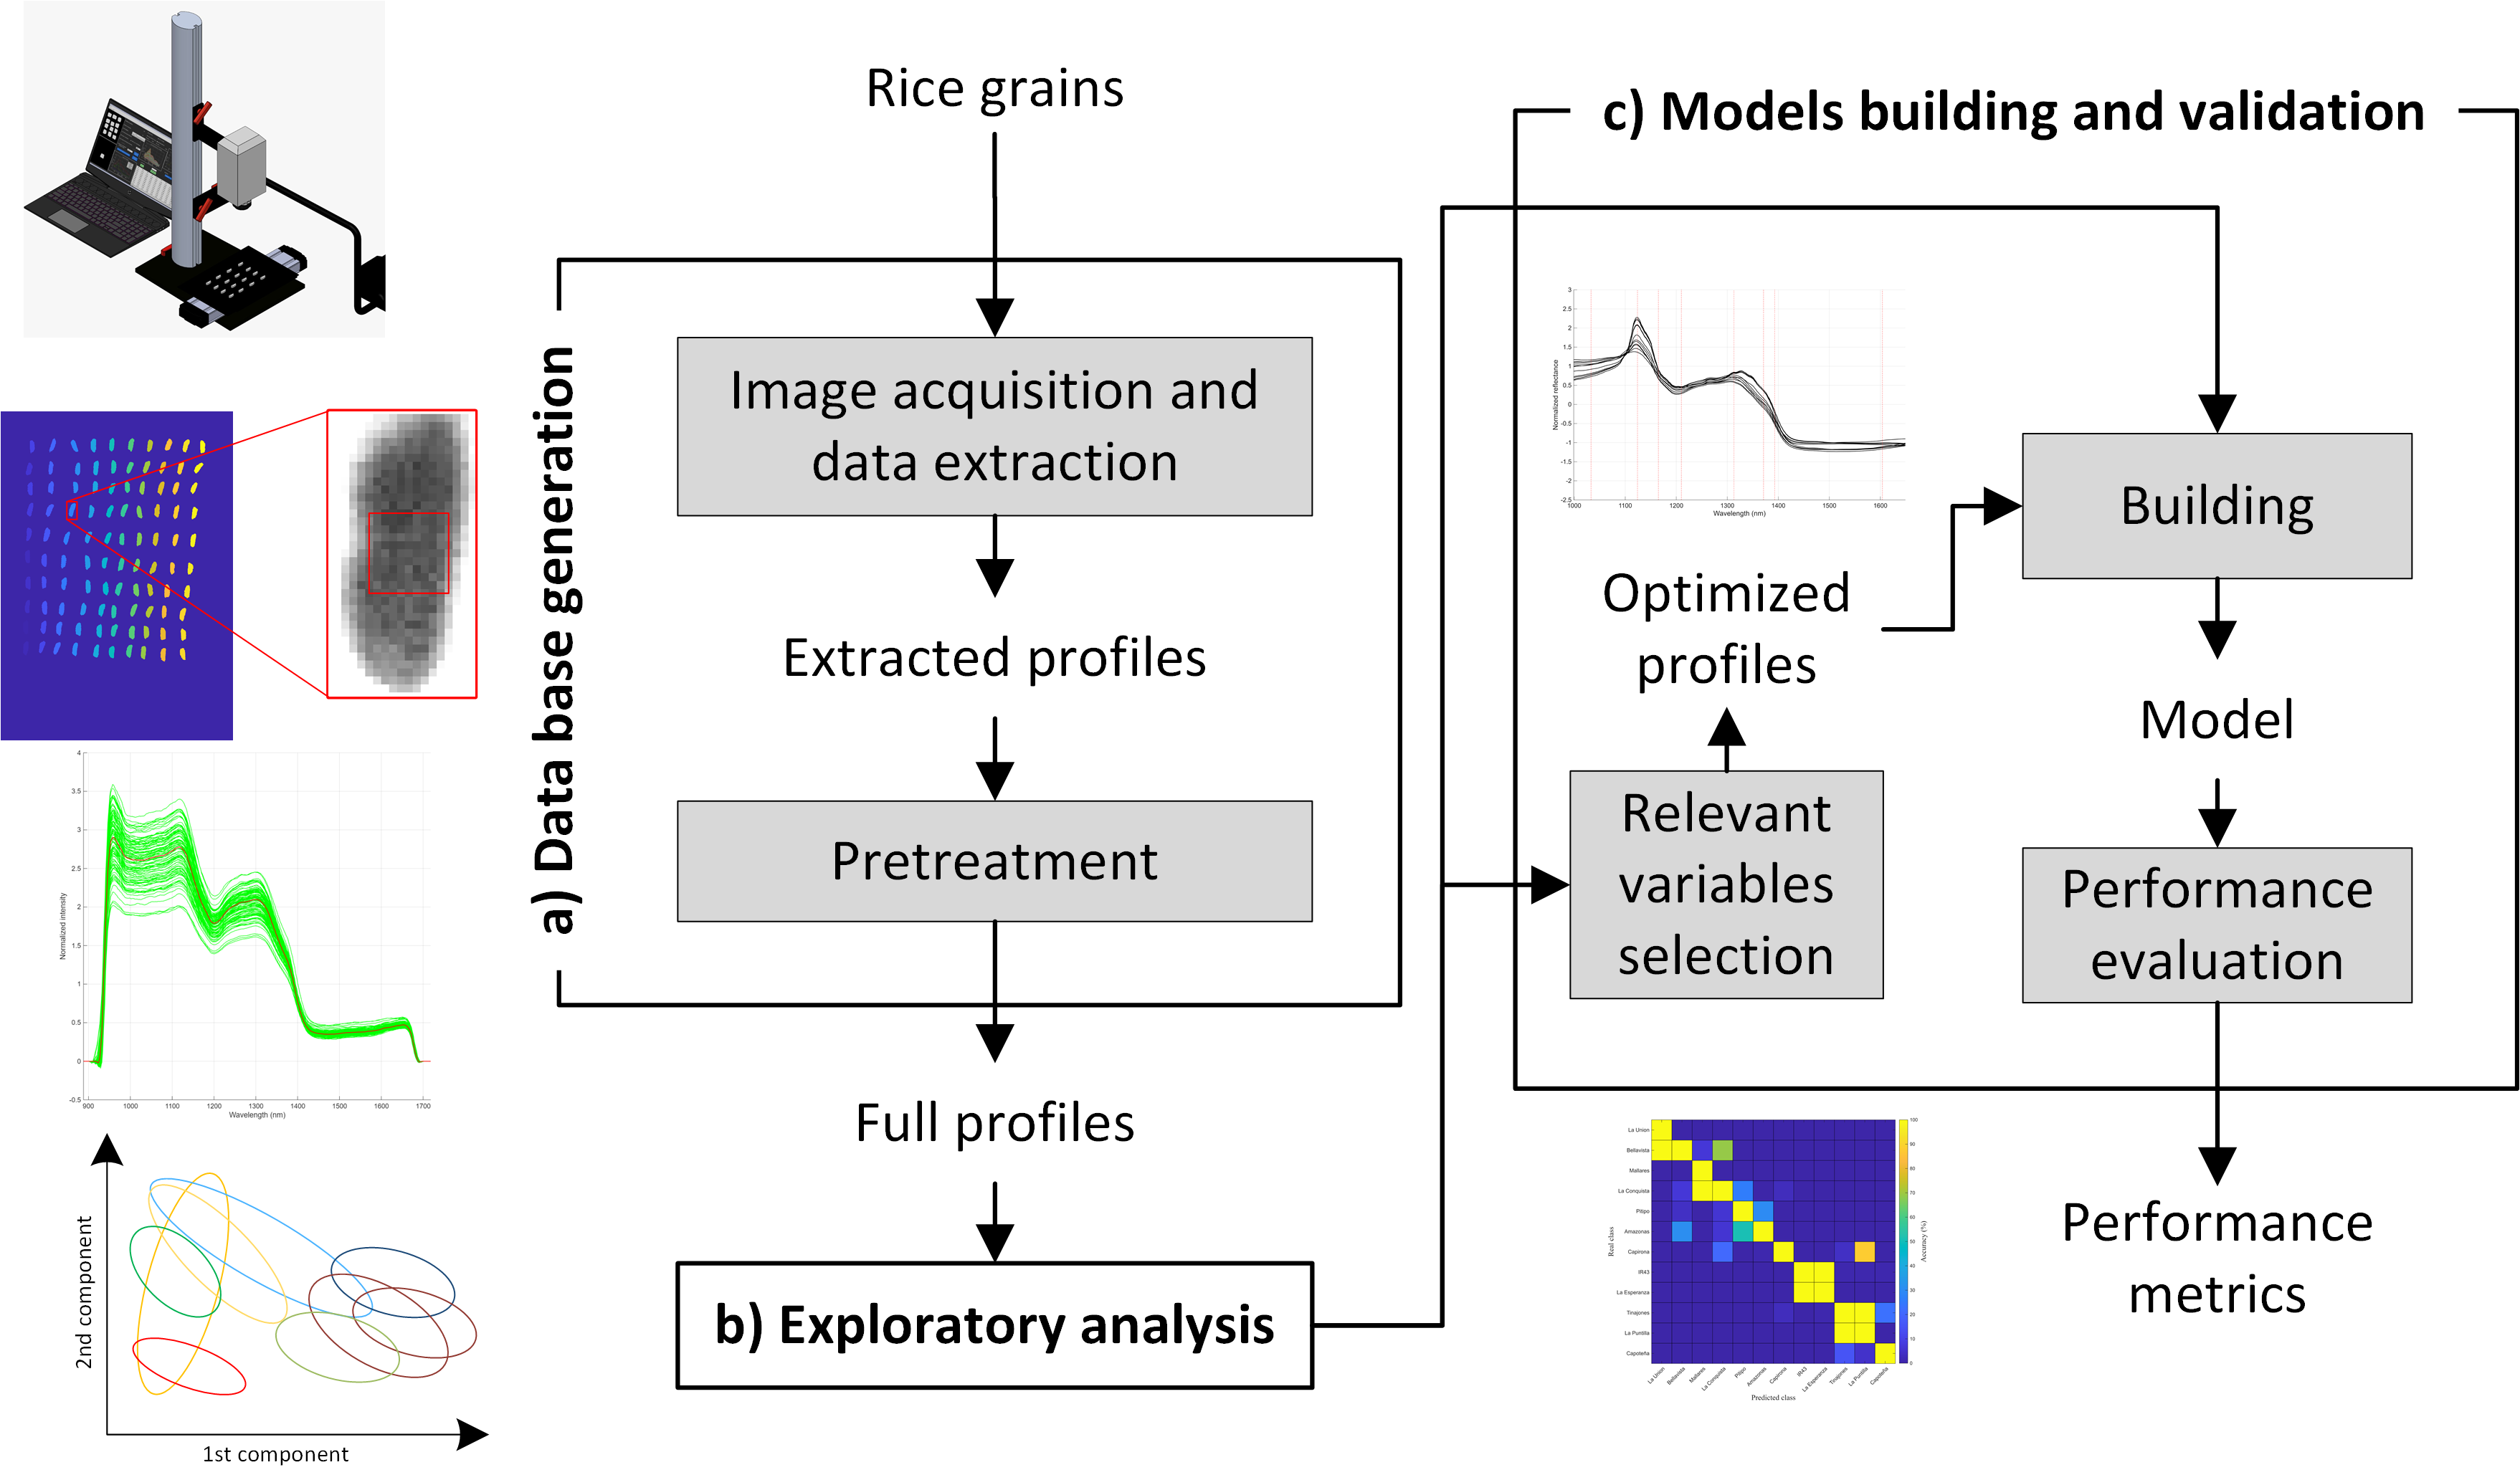
\includegraphics[width=0.75\textwidth]{Figures/Fig_01.png}
    \caption{Workflow of the study}
    \label{fig_01}
\end{figure*}


\subsection{Grains of rice}

% colecta de muestras

Half a kilogram of each of the twelve varieties was obtained from the National Institute of Agricultural Innovation (INIA) and transported to the Food Safety Research Laboratory of the National University of Frontera (UNF). The varieties were:  

\begin{multicols}{2}
\begin{itemize}
    \item La Unión
    \item Bellavista
    \item Mallares
    \item La Conquista
    \item Pitipo
    \item Amazonas
    \columnbreak
    \item Capirona
    \item IR43
    \item La Esperanza
    \item Tinajones
    \item La Puntilla
    \item Capoteña
\end{itemize}
\end{multicols}

The samples were stored in hermetically sealed dark bags under controlled environmental conditions (24 °C, dry environment) to maintain their spectral integrity until image acquisition.

\subsection{Database generation}\label{sec_database}

\subsubsection{Image acquisition and data extraction} 

% sobre el euipo y condiciones de toma de imagenes
Hyperspectral data were acquired using a Resonon Pika NIR-640 camera (Resonon Inc., USA) in reflectance mode (336 bands, 888--1718~nm; the analysis uses the 263 contiguous bands 47--309, 999--1649~nm); 500 grains of each rice variety were placed on a dark matte surface and imaged in blocks of 100 grains at a time. Each variety is a single lot, imaged in one session.
Acquisition was performed under controlled lighting conditions to achieve spectral stability and comparability between measurements.
The data, in band-interleaved-by-line (BIL) format, were stored on network-attached storage (NAS) for subsequent analysis. 

% sobre la extraccion de  los perfiles
Routines and functions were implemented to visualize the information contained in the hypercubes; the intensity image at 1475~nm, which gave the best contrast between grain and background, was used to segment the grains.
A square region of interest (ROI) measuring 11 pixels per side was generated based on the center of gravity of each grain, and the mean spectral profile was extracted from it.
The mean profile of each grain, coded by variety, was stored in a spreadsheet.
\added{The 500 rows of each variety in this matrix are taken to be its five images of 100 grains, in acquisition order; the image defines the unit of the grouped validation (Section~\ref{sec_building}).}

\subsubsection{Pre-treatment}

Raw hyperspectral data often contain noise due to instrumental and environmental effects \citep{vasquez2018}; therefore, the following pre-treatment steps were applied to each profile during extraction, before any of the analyses below.

\begin{itemize}
    \item \textbf{Smoothing.} For noise reduction, the Savitzky--Golay (SG) filter was applied; this filter preserves the shape of the peaks and reduces high-frequency noise; see Equation~\ref{eq_01}.
    \begin{equation}
        y_{i,j} = \sum_{k=-m}^{m} c_{k}\, x_{i,\,j+k}
        \label{eq_01}        
    \end{equation}
    where $y_{i,j}$ is the smoothed value of the sample $i$ at the wavelength index $j$; $x_{i,\,j+k}$ is the original value of the signal; $c_{k}$ are the SG convolution coefficients determined by the degree of the polynomial $p$ and the order of the derivative $d$; $m = (w-1)/2$ is the half-width of the window; and $w$ is the total length of the window (an odd number of points), which corresponds to $w = 2m + 1$. A window of $w=11$ points, polynomial degree $p=2$ and $d=0$ (smoothing only) were used, applied to the full 336-band profile.

    \item \textbf{Normalization.} The Z-score normalization method was applied to the profiles, scaling the data points so that they have a mean $(\mu)$ of 0 and a standard deviation ($\sigma$) of 1 over the full 336-band profile, before the 263 analyzed bands were taken, see Equation~\ref{eq_02}.
    \begin{equation}
        X_{Norm} = \frac{X-\mu}{\sigma}
        \label{eq_02}
    \end{equation}
     where $X_{Norm}$ is the normalized profile, $X$ the smoothed profile, and $\mu$ and $\sigma$ the mean and standard deviation of that profile.
\end{itemize}

\subsection{Exploratory analysis}

As in previous studies \citep{amigo2013,zhang2022,ali2024}, principal component analysis (PCA) was performed on the column-centered matrix of pre-treated profiles (singular value decomposition in NumPy).
The projection of the observations onto the first two principal components was visualized through a scatter plot, using distinct colors and markers per class, with confidence ellipses superimposed to assess dispersion and overlap between groups. 
To locate where the varieties differ, the standard deviation of the twelve variety means was divided at each band by the mean within-variety standard deviation (a per-band Fisher-type ratio).

\subsection{Model building and validation}

Modeling comprised three stages: (i) building and cross-validating four classifiers on the full spectrum; (ii) selecting bands with three methods and comparing each selection with random subsets of the same size; and (iii) evaluating performance from pooled confusion matrices, overall accuracy and the macro-averaged F1-score.


\subsubsection{Classifiers and cross-validation}\label{sec_building}

The classifiers were built and validated by five-fold cross-validation repeated six times (30 splits); each split tests 20\% of the grains of each variety, and every grain is tested six times. Two divisions were compared. In the \emph{random division}, individual grains were assigned to folds at random within each variety, as is usual in the field. In the \emph{grouped division}, whole images of 100 grains were assigned to folds, so that each split holds out one image per variety and grains imaged together never appear on both sides; the images of each variety were shuffled independently in each repetition, so that the twelve held-out images are combined differently in every split. The random division estimates accuracy on grains from images already seen during training; the grouped division estimates accuracy on grains from another image of the same lot. Band standardization, where used, was fitted on the training part of each split.

\begin{itemize}
    \item[(a)] Linear discriminant analysis (LDA).
    This model, see Figure~\ref{fig_models}a, seeks a linear combination of variables that provides discrimination between classes \citep{Rahmani2022}.
    \added{It was fitted as a single multiclass model with a pooled covariance matrix (scikit-learn \texttt{LinearDiscriminantAnalysis}).}
    \item[(b)] \added{Linear SVM on unstandardized bands (L-SVM): one-vs-one binary linear SVMs with hinge loss and $C=1$ (scikit-learn \texttt{LinearSVC} in a \texttt{OneVsOneClassifier}), fitted to convergence. It differs from the SVM below in the absence of standardization and in the solver (liblinear, which also penalizes the intercept, rather than libsvm).}
    \item[(c)] Linear support vector machine (SVM).
    This model constructs a separating hyperplane whose position is set by maximizing the margin to the closest samples, the support vectors (Figure~\ref{fig_models}b). 
    In addition, kernel functions can be used to address nonlinear classification problems \citep{Onmarkhong2022, castro2019}.
    A multiclass SVM with a linear kernel ($C=1$, one-vs-one) was fitted on standardized bands (scikit-learn \texttt{SVC} after \texttt{StandardScaler}).
    \item[(d)] Artificial neural network (ANN).
    In this case, interconnected processing units, called neurons, are organized into layers and learn nonlinear relationships between input variables and outputs by adjusting connection weights. 
    In a backpropagation network, learning involves forward propagation of information followed by backward propagation of the prediction error to update the network parameters (Figure~\ref{fig_models}c) \citep{Kang2024, castro2019}.
    A feed-forward network with standardized inputs and a single ReLU hidden layer of \added{$\mathrm{round}(\sqrt{p})$} neurons, $p$ being the number of bands (16 for the full spectrum, 3 for nine bands), was trained with L-BFGS (scikit-learn \texttt{MLPClassifier}; at most 1000 iterations, L2 penalty $10^{-4}$).
\end{itemize}

\begin{figure}[htbp!]
    \centering
    \subfloat[]{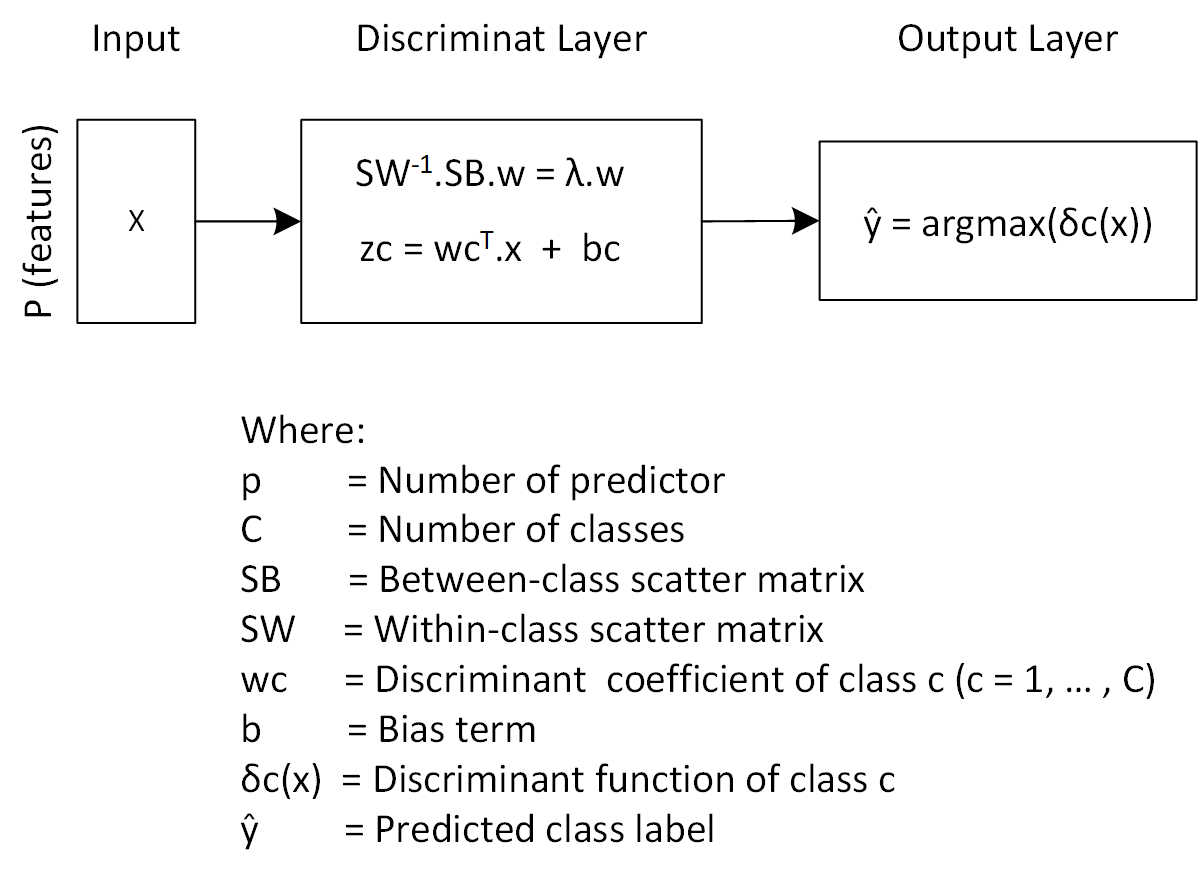
\includegraphics[width=0.85\columnwidth]{Figures/model_LDA.png}}\\ 
    \subfloat[]{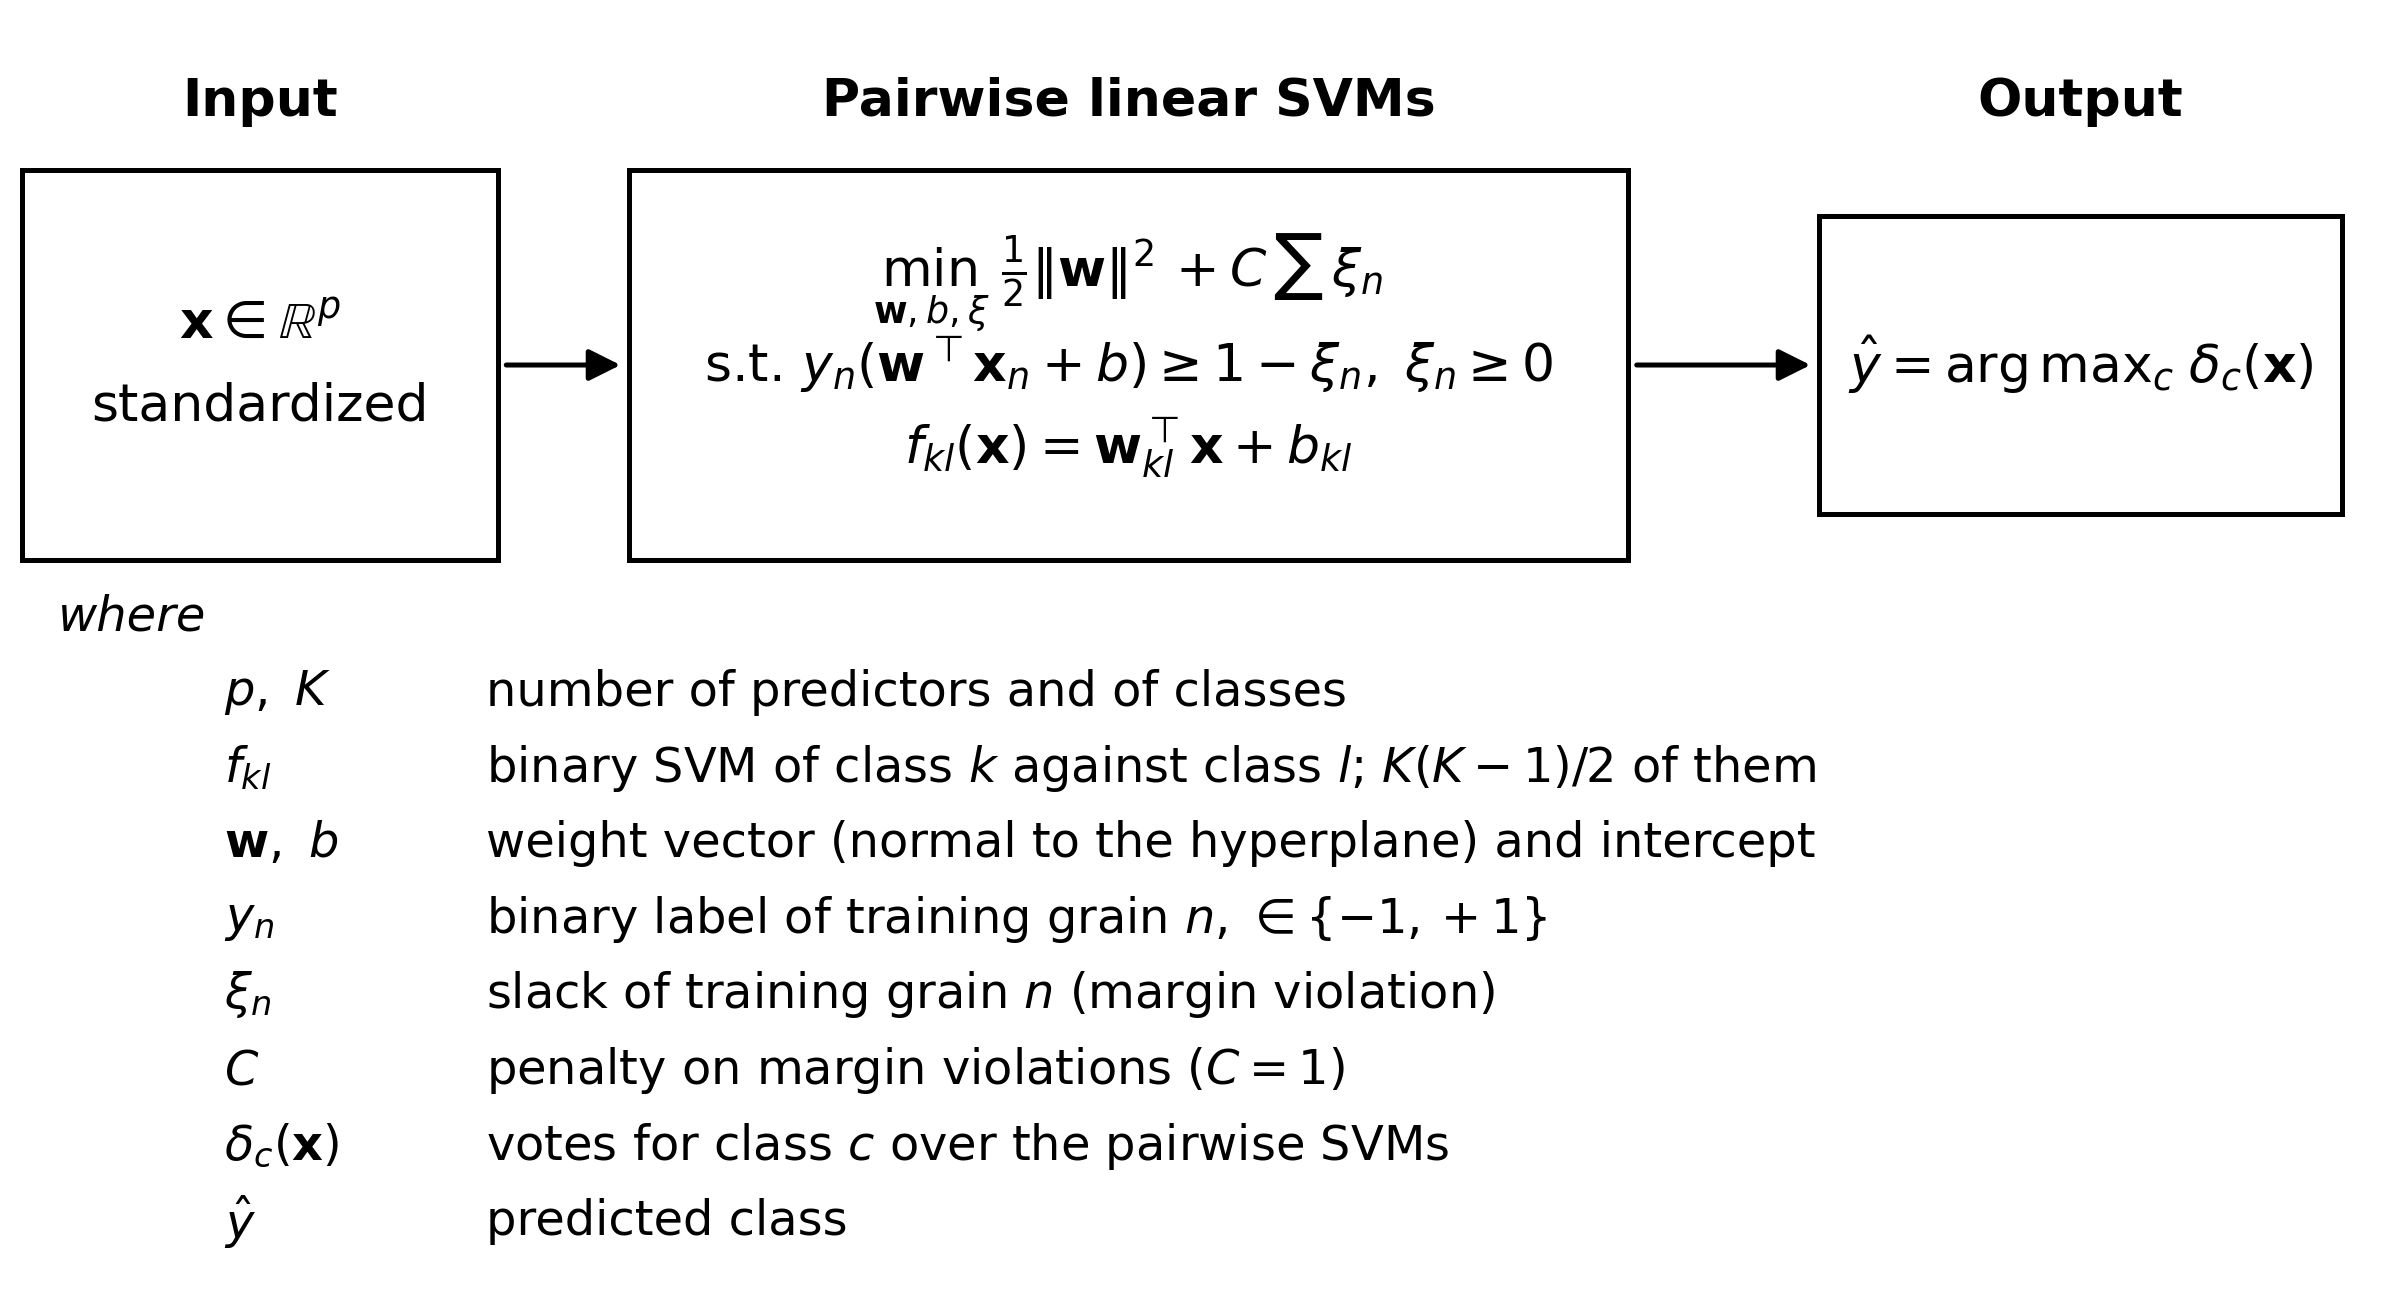
\includegraphics[width=0.85\columnwidth]{Figures/model_SVM.png}}\\
    \subfloat[]{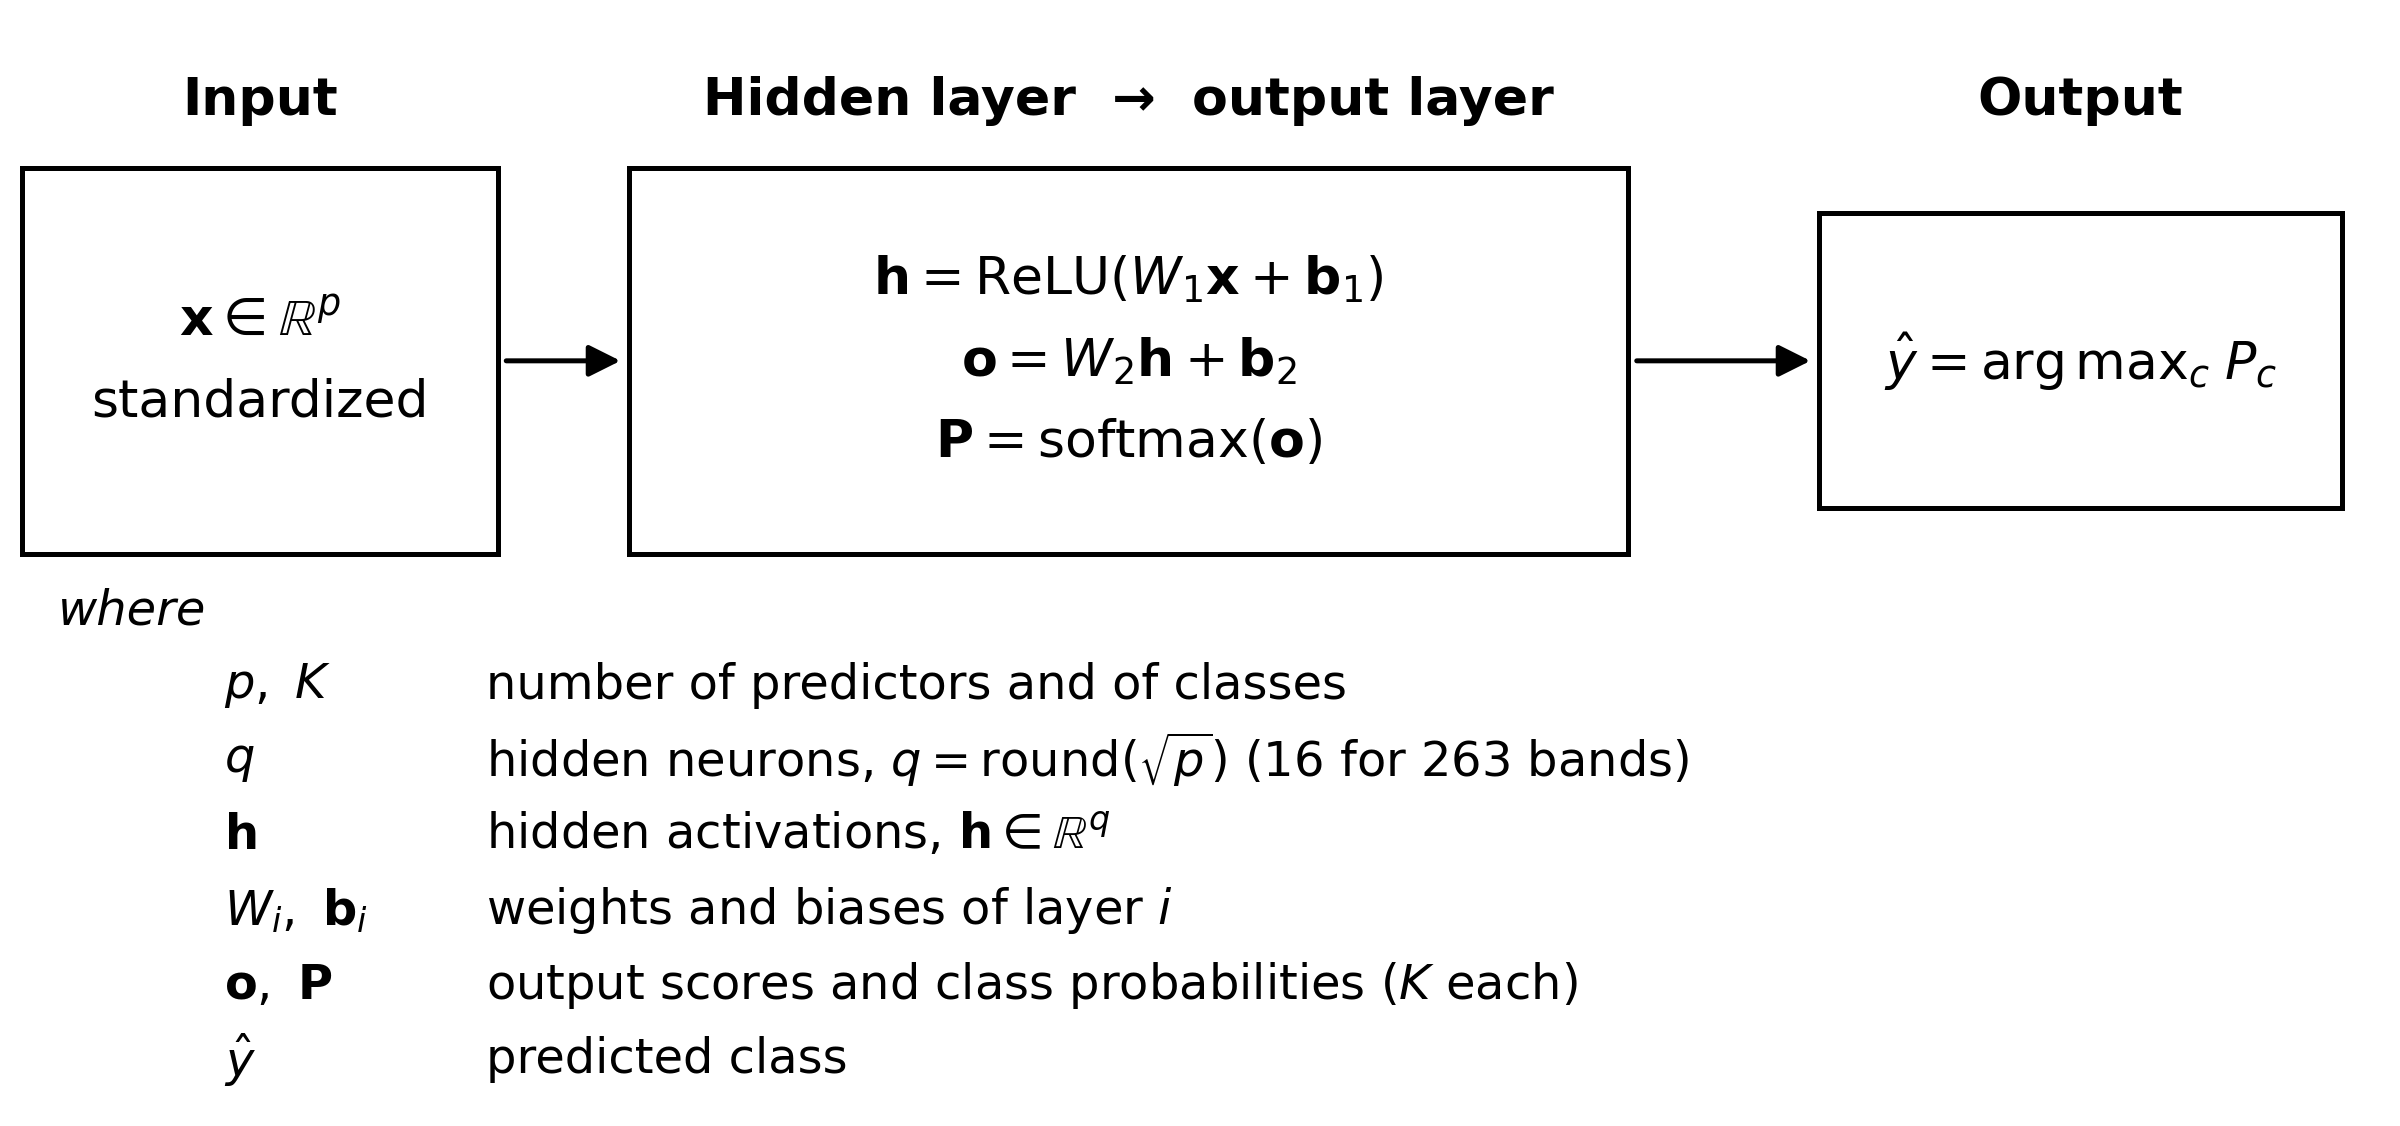
\includegraphics[width=0.85\columnwidth]{Figures/model_ANN.png}} 
    \caption{Schematic diagrams of the (a) LDA, (b) SVM and (c) ANN classifiers}
    \label{fig_models}
\end{figure}


\subsubsection{Band selection}\label{sec_feature_selection}

Three alternative feature selection strategies were implemented to identify the most relevant spectral bands and to compare their effect on classification performance \citep{Rahmani2022, Castro2022cafs}: 

\begin{itemize}
    \item[--] Feature selection by neighborhood component analysis (FSCNCA).
    This supervised method assigns a weight to each feature based on its contribution to prediction. 
    Features with larger weights are considered to be more relevant, whereas features with small weights can be removed to obtain a reduced representation of the original feature space.
    \added{Feature-weighted NCA \citep{Yang2012nca} was implemented in Python: a weight per band, distance $D_{ij}=\sum_r w_r^2|x_{ir}-x_{jr}|$, kernel width $\sigma=1$, regularization $\lambda=1/n$, weights initialized at 1 and optimized by gradient ascent (Adam, learning rate 0.02, 150 iterations) on a random subsample of 100 standardized profiles per variety, to bound the cost of the pairwise terms. The bands were ranked by their weight and the $k$ largest retained.}
    
    \item[--] Sequential forward selection (SFS).
    This is a wrapper-based method that starts with an empty feature subset and sequentially adds the feature that produces the greatest improvement according to a predefined model-performance criterion.
    The process progressively constructs a reduced feature subset without exhaustively evaluating all possible combinations. 
    The implementation uses LDA as the evaluation model: starting from an empty set, it evaluates every remaining band at each step and adds the one that maximizes the mean five-fold cross-validated accuracy; the inner folds are formed from blocks of 10 consecutive grains, so that neighboring grains are not split between fitting and scoring. The first $k$ bands added are retained.

    \item[--] Covering array feature selection (CAFS).
    It is a supervised wrapper approach based on covering arrays, combinatorial structures characterized by high interaction coverage with a reduced number of configurations. 
    CAFS uses the subset of experiments defined by the covering array to explore the feature space and identify the features that maximize a predictive-performance criterion, such as the F1-score.
    This enables the exploration of relevant feature interactions with substantially fewer combinations than an exhaustive search.
    The implementation is based on previously reported work by \citet{Castro2022cafs}, and uses a Gaussian naive Bayes classifier scored by the macro-averaged F1-score in an inner five-fold cross-validation \added{(folds formed from blocks of 10 consecutive grains, as for SFS)}. \added{It was ported line by line to Python from the MATLAB code of \citet{Castro2022cafs} (binary covering arrays of strength 2; our generator reproduces theirs exactly). At each iteration the current band set is split according to the rows of the covering array, the best-scoring row becomes the new set, and the best subset over all iterations is returned; CAFS therefore sets its own subset size.}
    The algorithm was configured with the following options: 
    \begin{itemize}
        \item  Patience parameter (Patience = 3)
        \item  Minimum improvement threshold (MinImprovement = $10^{-4}$)
        \item  Subset size at or below which the search stops (MinFeatures = 10; the last iteration can fall below it) 
        \item  Maximum number of iterations (MaxIterations = 50)
        \item  Target number of features (TargetFeatures = 20)
        \item  Compactness penalty (CompactnessPenalty = 0.10)
        \item  Exponent of the excess penalty (ExcessPenaltyPower = 2)
        \item  Scale of the adaptive penalty (AdaptivePenaltyAlpha = 2)
    \end{itemize}

     The original implementation applies standard normal variate (SNV) to each profile; SNV coincides with the Z-score normalization already applied (Equation~\ref{eq_02}), so it has no further effect here. The compactness penalty discourages subsets larger than the target size.
        
\end{itemize}

\added{\textbf{Two uses of selection.} Each method was applied in two ways. (1) \emph{Once on all spectra}: SFS and FSCNCA retaining $k=9$ bands, and CAFS with its own subset size, fitted on all 6000 profiles, as is common in the field. The test grains then take part in choosing the bands, which favors these subsets \citep{Varma2006}; they are evaluated to show how large this advantage is. (2) \emph{Within training}: each method fitted on the training part of a split only, so that the test grains take no part in choosing the bands; SFS and FSCNCA at $k\in\{5,10,20,40\}$ and CAFS with its own size, on 10 splits (two repetitions of the grouped five-fold cross-validation, drawn independently of the 30 splits of Table~\ref{tab:acc}), with any internal cross-validation grouped in blocks of 10 rows. The subsets were evaluated on the test part with the SVM and LDA; the ANN and the L-SVM were left out to limit the cost (1200 fits per classifier and method).}
\added{\textbf{Random-subset baseline.} Because neighboring NIR bands are strongly correlated, a small set of bands drawn at random may already carry most of the discriminant information. To judge whether a selection method identifies informative bands, rather than merely reducing their number, every selected subset was compared on the same split, with one image per variety held out, against 30 subsets of the same size drawn uniformly at random from the 263 bands.}

\subsubsection{Performance evaluation}\label{sec_performance}

The classification performance was evaluated through two complementary procedures: 

\begin{itemize}
    \item [-] Generation of average confusion matrices. 
    For each split a confusion matrix was computed, and the 30 matrices were pooled. 
    Each row of the pooled matrix was then normalized to percentages, which shows per-class performance independently of class size, and displayed as a heatmap.
   
    \item [-] Calculation of quantitative \added{per-class} metrics. For each split, the following quantities were derived from the confusion matrix: true positives (TP, diagonal elements), false positives (FP, column sums minus TP), false negatives (FN, row sums minus TP), and true negatives (TN, total minus (FP + FN + TP)). 
    From these, \added{three} standard metrics were calculated per class and per split: precision, defined as TP / (TP + FP); recall (sensitivity), defined as TP / (TP + FN); and the F1-score, defined as the harmonic mean 2·(Precision·Recall) / (Precision + Recall).
    The structure of the confusion matrix and these ratios are shown in Figure~\ref{figCM}, and the metrics were calculated in a way similar to \citet{castro2019}, see Equations~\ref{eq_acc} to \ref{eq_fm}\added{; Equation~\ref{eq_acc} is the overall accuracy over all classes, and Equations~\ref{eq_pre}--\ref{eq_fm} are per class}.

    \begin{figure}[htbp!]
        \centering
        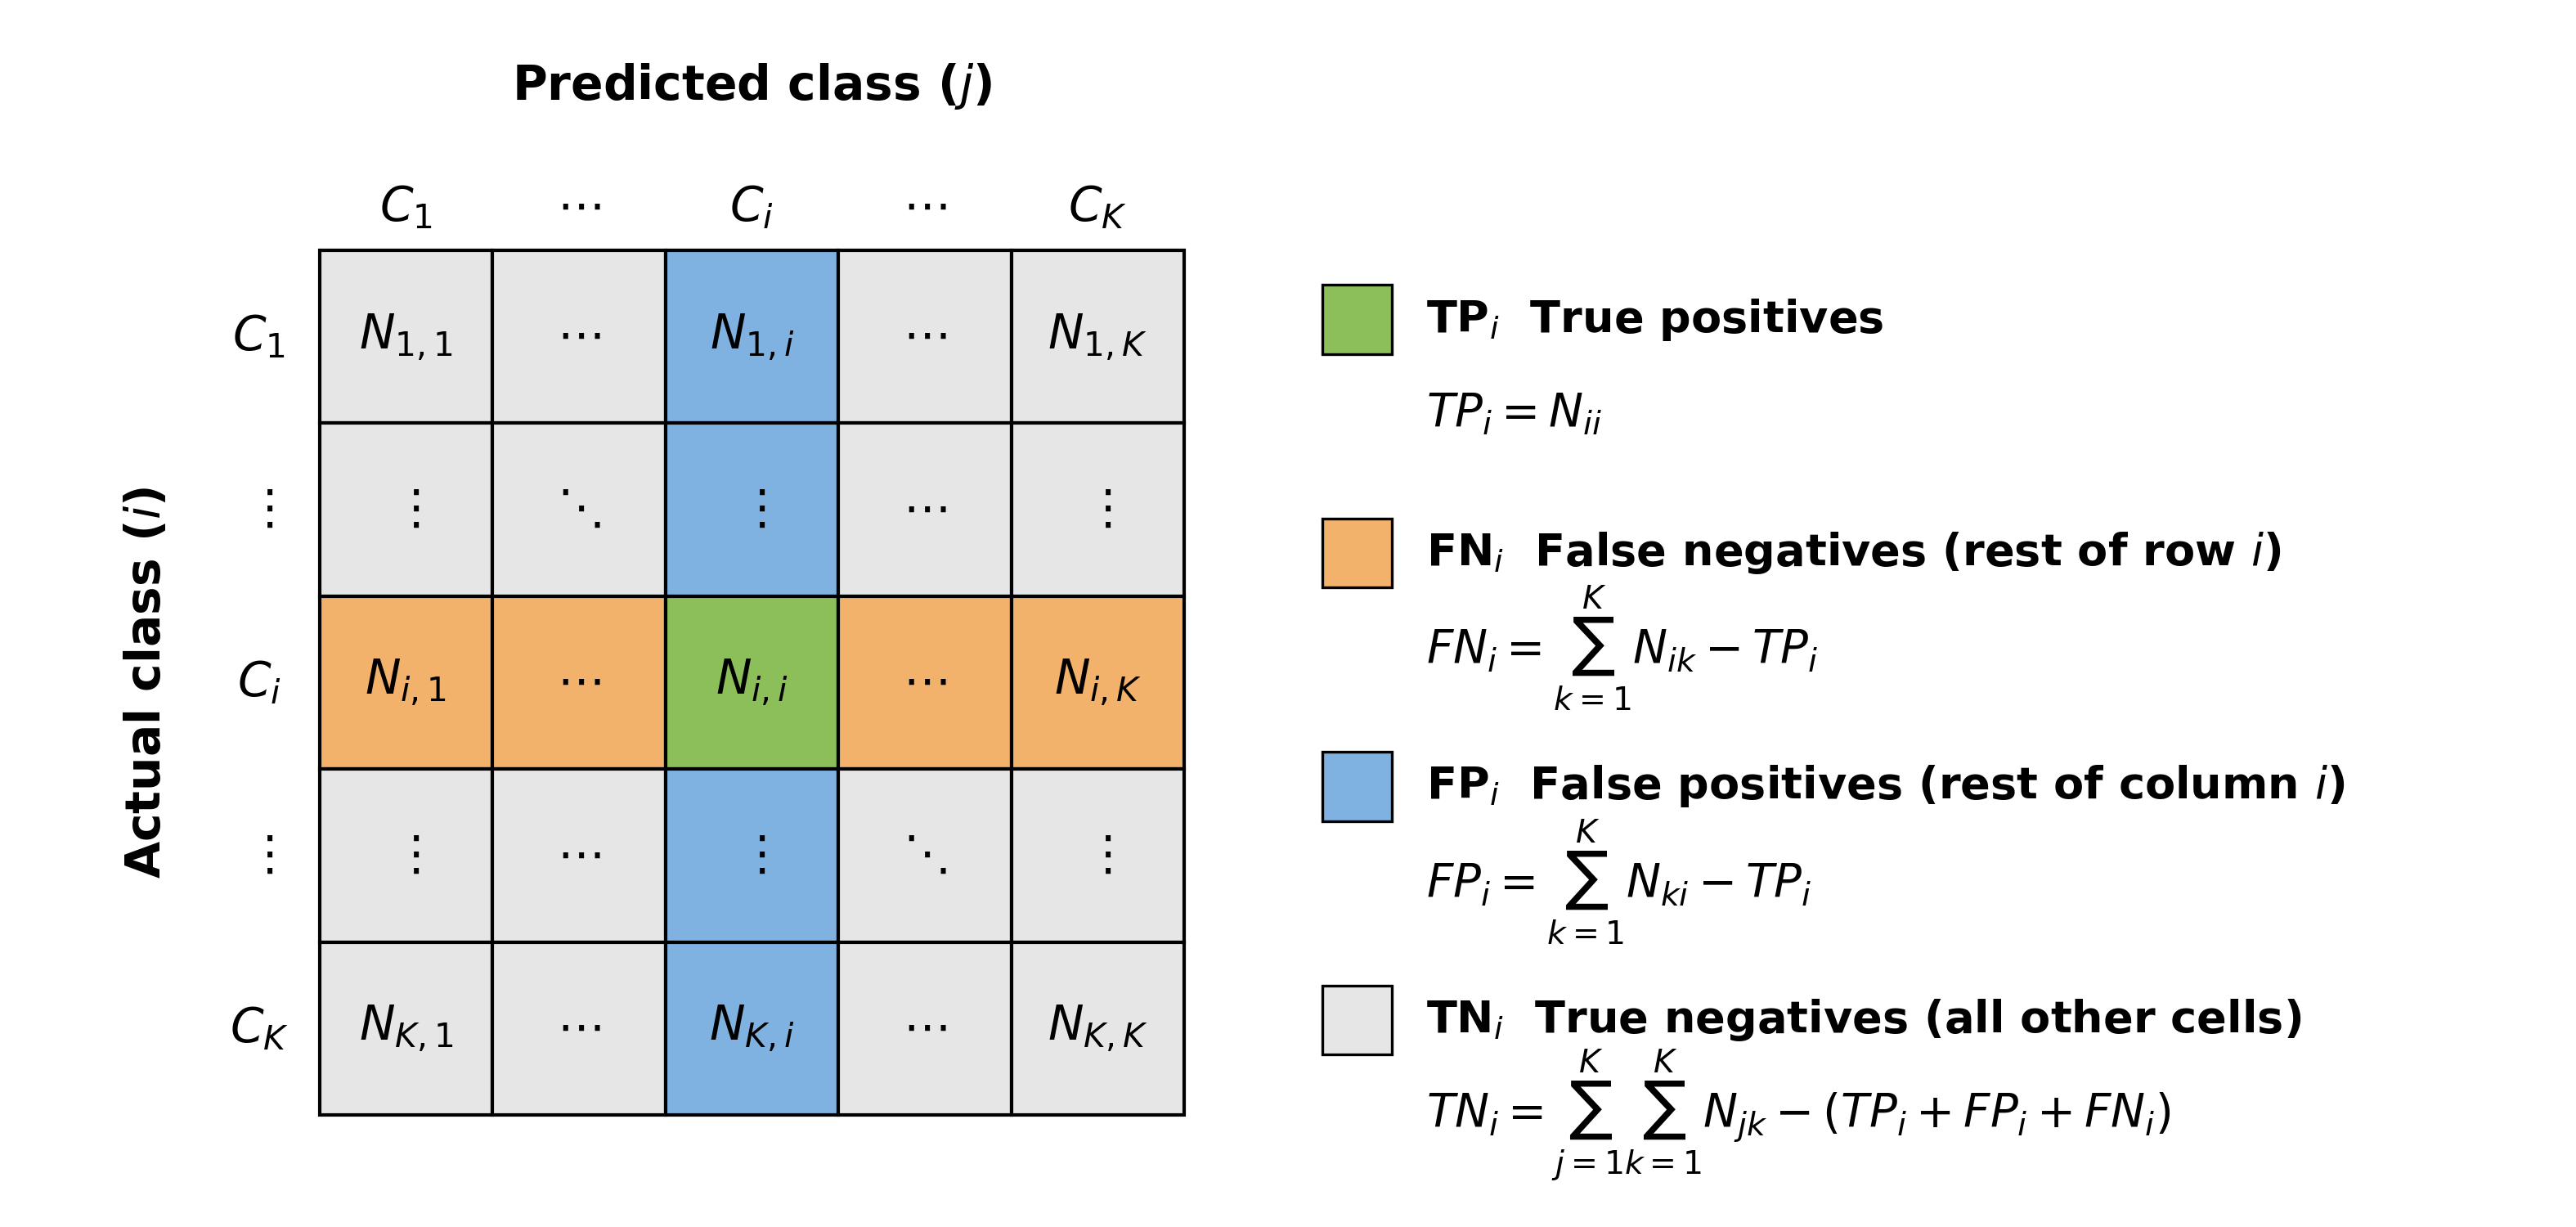
\includegraphics[width=1.0\columnwidth]{Figures/fig_CM.png}
        \caption{Structure of the confusion matrix and the quantities derived from it (TP, FP, FN, TN).}
        \label{figCM}
    \end{figure}

    \begin{equation}
        Accuracy \, (acc) = \frac{\sum_{i=1}^{K}TP_{i}}{\sum_{i=1}^{K} \sum_{j=1}^{K}N_{ij}}
        \label{eq_acc}
    \end{equation}
    \begin{equation}
        Precision \, (pre) = \frac{TP_{i}}{TP_{i} + FP_{i}}
        \label{eq_pre}
    \end{equation}
    \begin{equation}
        Recall \, (rec) =  \frac{TP_{i}}{TP_{i} + FN_{i}}
        \label{eq_rec}
    \end{equation}
    \begin{equation}
        F\text{-}measure_{i} \, (FM) =  2\left(\frac{pre_{i}\cdot rec_{i}}{pre_{i}+rec_{i}}\right)
        \label{eq_fm}
    \end{equation}
    where $N_{ij}$ is the number of grains of variety $i$ assigned to variety $j$.
\added{Overall accuracy (Equation~\ref{eq_acc}) is the primary metric, reported together with the macro-averaged F1-score. The per-class one-vs-rest accuracy $(\mathrm{TP}+\mathrm{TN})/N$ was not used as a summary: with $K$ classes and overall error $e$, its mean over classes equals $1-2e/K$ exactly, whatever the class balance, because every misclassified grain counts once as a false negative and once as a false positive. It therefore carries no information beyond overall accuracy, compresses differences by a factor $K/2$, and cannot fall below $1-2/K$: for $K=12$ an overall accuracy of 97\% appears as 99.5\%, random guessing scores 84.7\%, and a classifier that is always wrong still scores 83.3\%.}
    For each metric, the mean and standard deviation over the \added{30 splits} were calculated; this procedure was repeated for each classifier and each feature configuration considered in the study (full spectrum and each selected subset).
    \added{Statistical comparisons (Sections~\ref{sec_classification} and \ref{sec_bands_results}) were made as follows. The 30 splits reuse the same 60 images, so they are not independent observations and tests on them overstate the evidence \citep{Nadeau2003}. Classifiers were therefore compared at the level of images: the accuracy of each image was averaged over the repetitions in which it was tested, the classifiers were compared in pairs over the 60 images with the Wilcoxon signed-rank test, and 95\% confidence intervals for the differences were obtained by resampling images (10\,000 bootstrap samples); random and grouped division were compared in the same way, paired by image. Band subsets were compared with random subsets on each split (paired $t$-test and Wilcoxon test over the splits); these comparisons share the same limitation, so their $p$-values indicate how consistent a difference is across splits rather than giving formal evidence. $P$-values were adjusted with the Holm procedure within each family (12 classifier comparisons; 4 drops from random to grouped division; 12 comparisons of the subsets selected once on all spectra with random subsets; 30 comparisons of training-only selections with random subsets), and a difference is reported as significant at an adjusted $p<0.05$.}

\end{itemize}



% ================================================================================================
%% RESULTS AND DISCUSSIONS
% ================================================================================================

\section{Results}

\subsection{Mean profiles}\label{sec_mean_profiles}

\begin{figure}[htbp!]
    \centering
    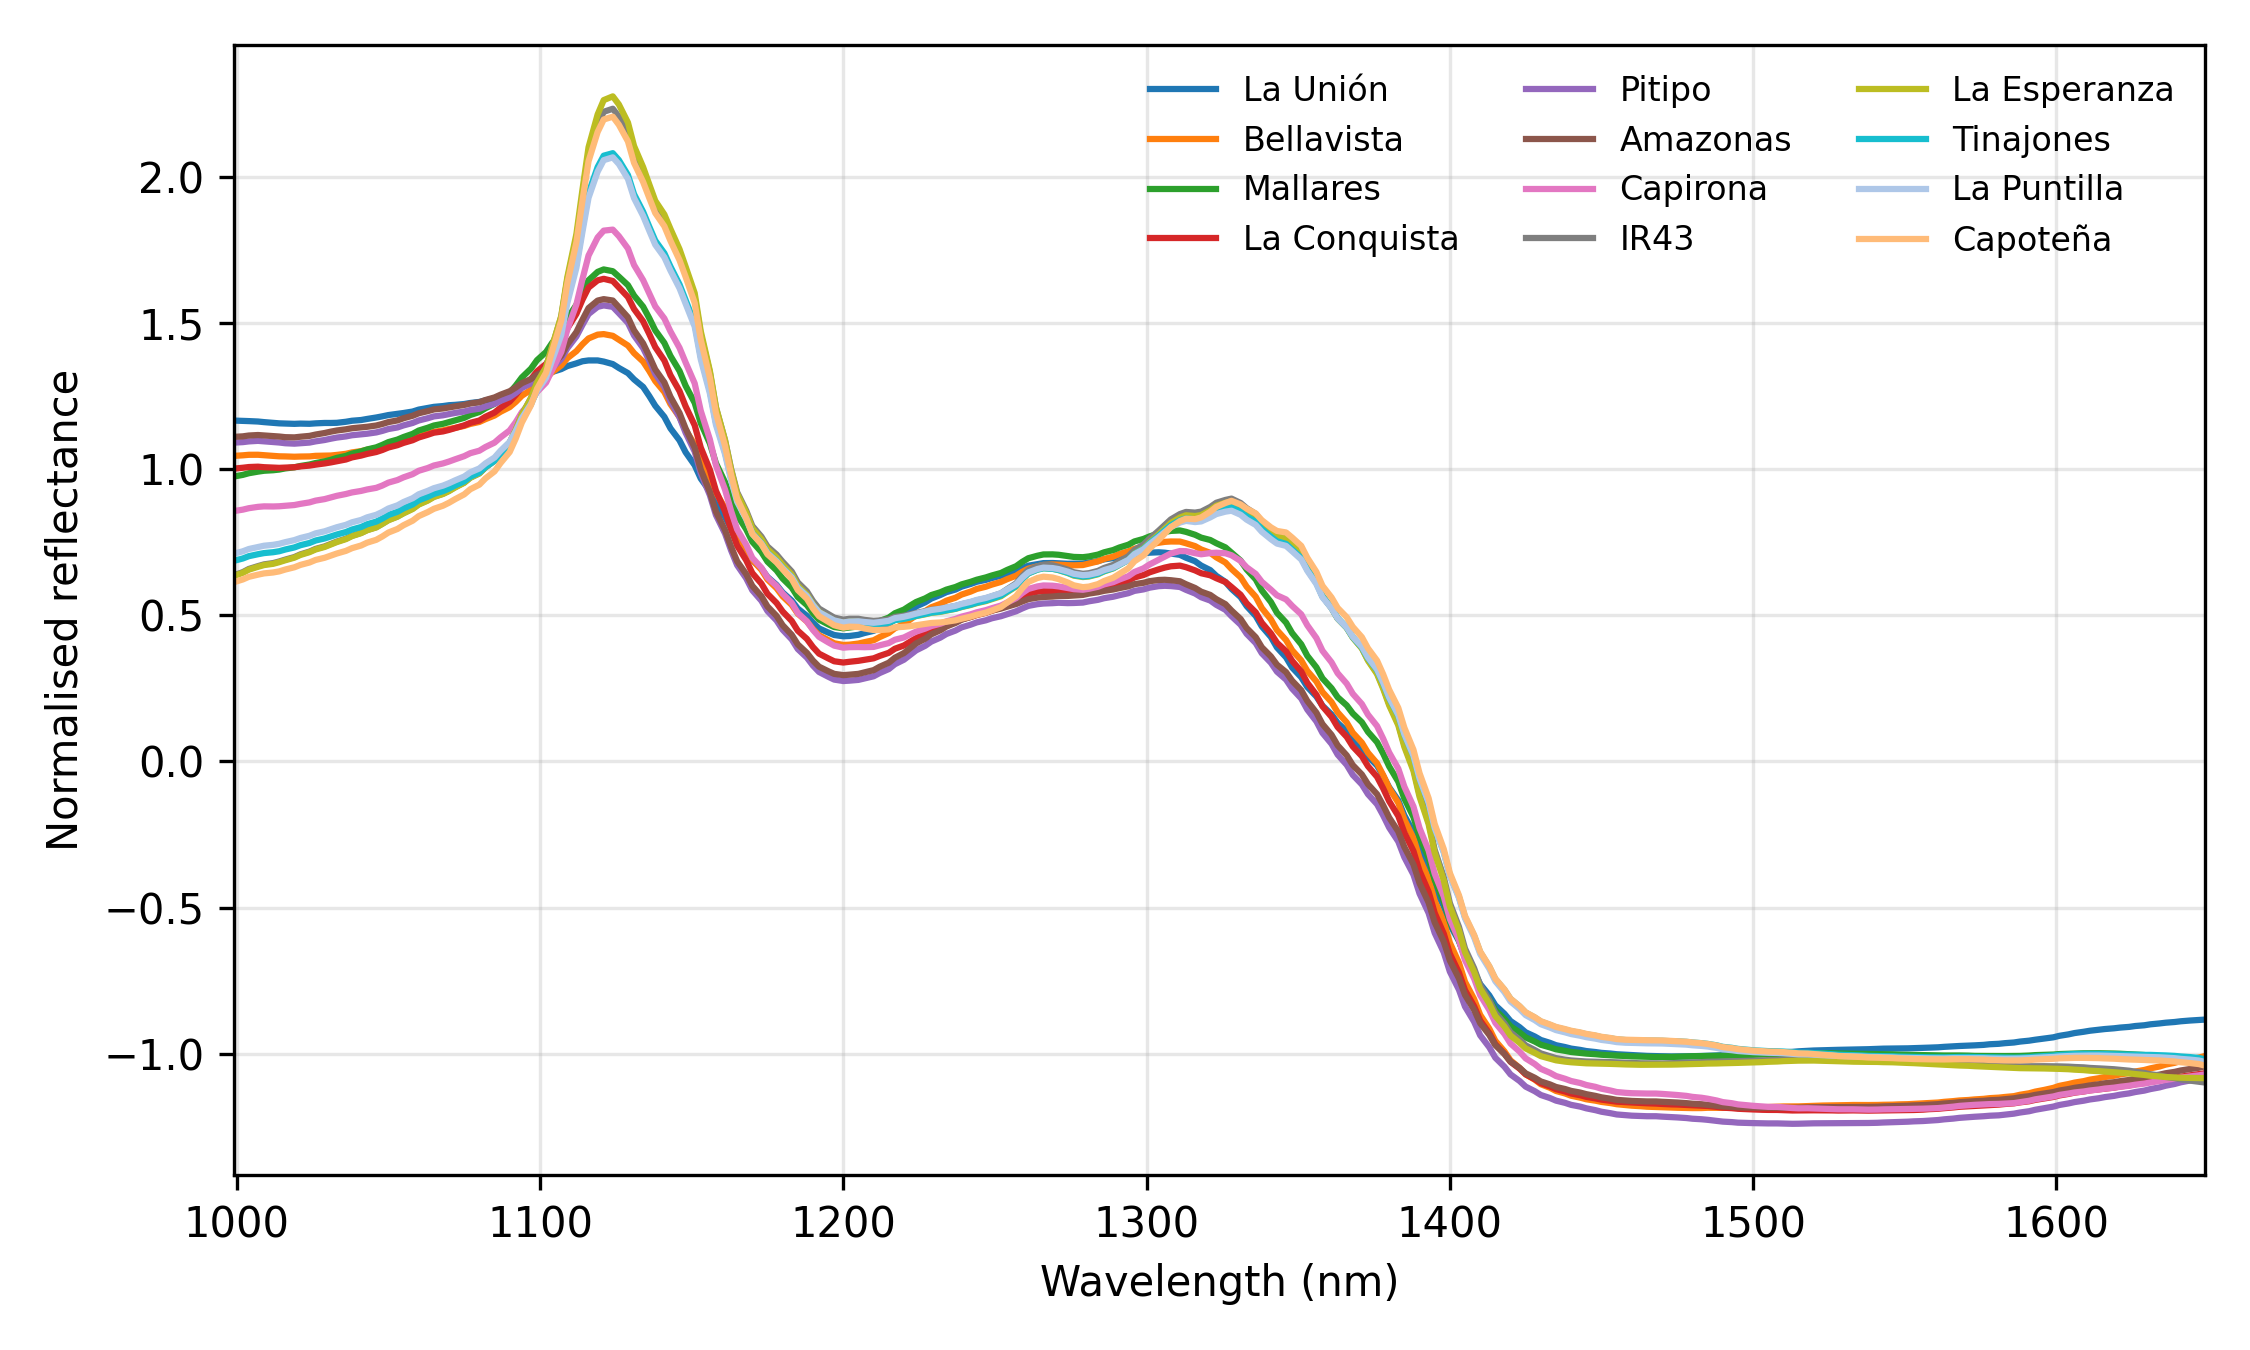
\includegraphics[width=\columnwidth]{Figures/fig_py_perfiles.png}
    \caption{Mean pre-treated (Savitzky--Golay smoothed, Z-score normalized) profile of each of the twelve varieties over the 263 bands (999--1649~nm).}
    \label{fig_02}
\end{figure}

\added{Figure~\ref{fig_02} shows the mean profile of each variety after Savitzky--Golay smoothing and Z-score normalization. The profiles are reflectance, so absorption bands appear as minima and as the falling edges that lead into them, while maxima are windows of comparatively weak absorption between bands. All twelve profiles share the same shape: a rising edge from 1000~nm to a reflectance maximum near 1120--1125~nm, a sharp fall to a minimum near 1195--1200~nm, a secondary maximum near 1300--1330~nm, a steep fall between about 1340 and 1430~nm, and a low, nearly flat plateau from 1430~nm to the end of the range near 1650~nm, where the varieties differ little. Varieties differ mainly in amplitude rather than in position: the highest maxima near 1120 and 1300~nm belong to the same two or three varieties throughout, and the lowest to a different, consistent subset. In this range the varietal signal is therefore carried by the depth of the absorption features and the height of the windows between them, not by shifts in wavelength. Relative to the scatter between grains of the same variety, the varieties differ most on the falling edge between 1100 and 1150~nm, where the standard deviation of the variety means reaches six times the within-variety one (at 1141~nm), then on the fall between 1340 and 1430~nm and below 1100~nm, and least around the minimum near 1200~nm (ratio below 2) and on the plateau.}
\added{The minimum near 1195--1200~nm lies in the second-overtone region of C--H stretching of CH$_2$ and CH$_3$ groups \citep{Workman2012}. On rice grain, \citet{John2022nirs}, surveying 500 brown rice accessions, assign 1196~nm to ``the C--H second overtone corresponding to aliphatic hydrocarbons'', and \citet{Onmarkhong2022} assign 1202~nm to the second overtone of the symmetric C--H stretching of CH$_3$ groups, associated with amylose. The falling edge that leads into this minimum, from the maximum near 1125~nm, covers the band that \citet{Shao2011starch} found in second-derivative absorbance spectra of rice flour at 1131--1155~nm and assigned to C--H stretching of starch (they call it the first overtone; standard tables place C--H second overtones in this region \citep{Workman2012}). The C--H absorption near 1200~nm thus combines starch and lipid, and the single band does not by itself separate the two. The fall between 1340 and 1430~nm and the low plateau beyond it are the first-overtone O--H absorption of water, which \citet{Shao2011starch} place at 1418~nm in rice flour, together with C--H combination bands near 1360--1420~nm \citep{Workman2012}; the plateau also spans the first overtone of N--H stretching of protein near 1500--1530~nm and the O--H stretching of starch near 1580~nm \citep{Onmarkhong2022}. The maxima near 1120 and 1300~nm are not absorption bands: their height reflects how deep the neighboring bands are and how strongly the grain scatters. Band positions shift with the matrix, so we rely on the rice studies \citep{Shao2011starch,John2022nirs,Onmarkhong2022} for specific positions and use the general tables only at the level of spectral regions.}
The spectral differences between the twelve varieties are therefore consistent with differences in starch, lipid and water absorption (Section~\ref{sec_discussion}).

\subsection{Exploratory analysis}

\begin{figure}[htbp!]
    \centering
    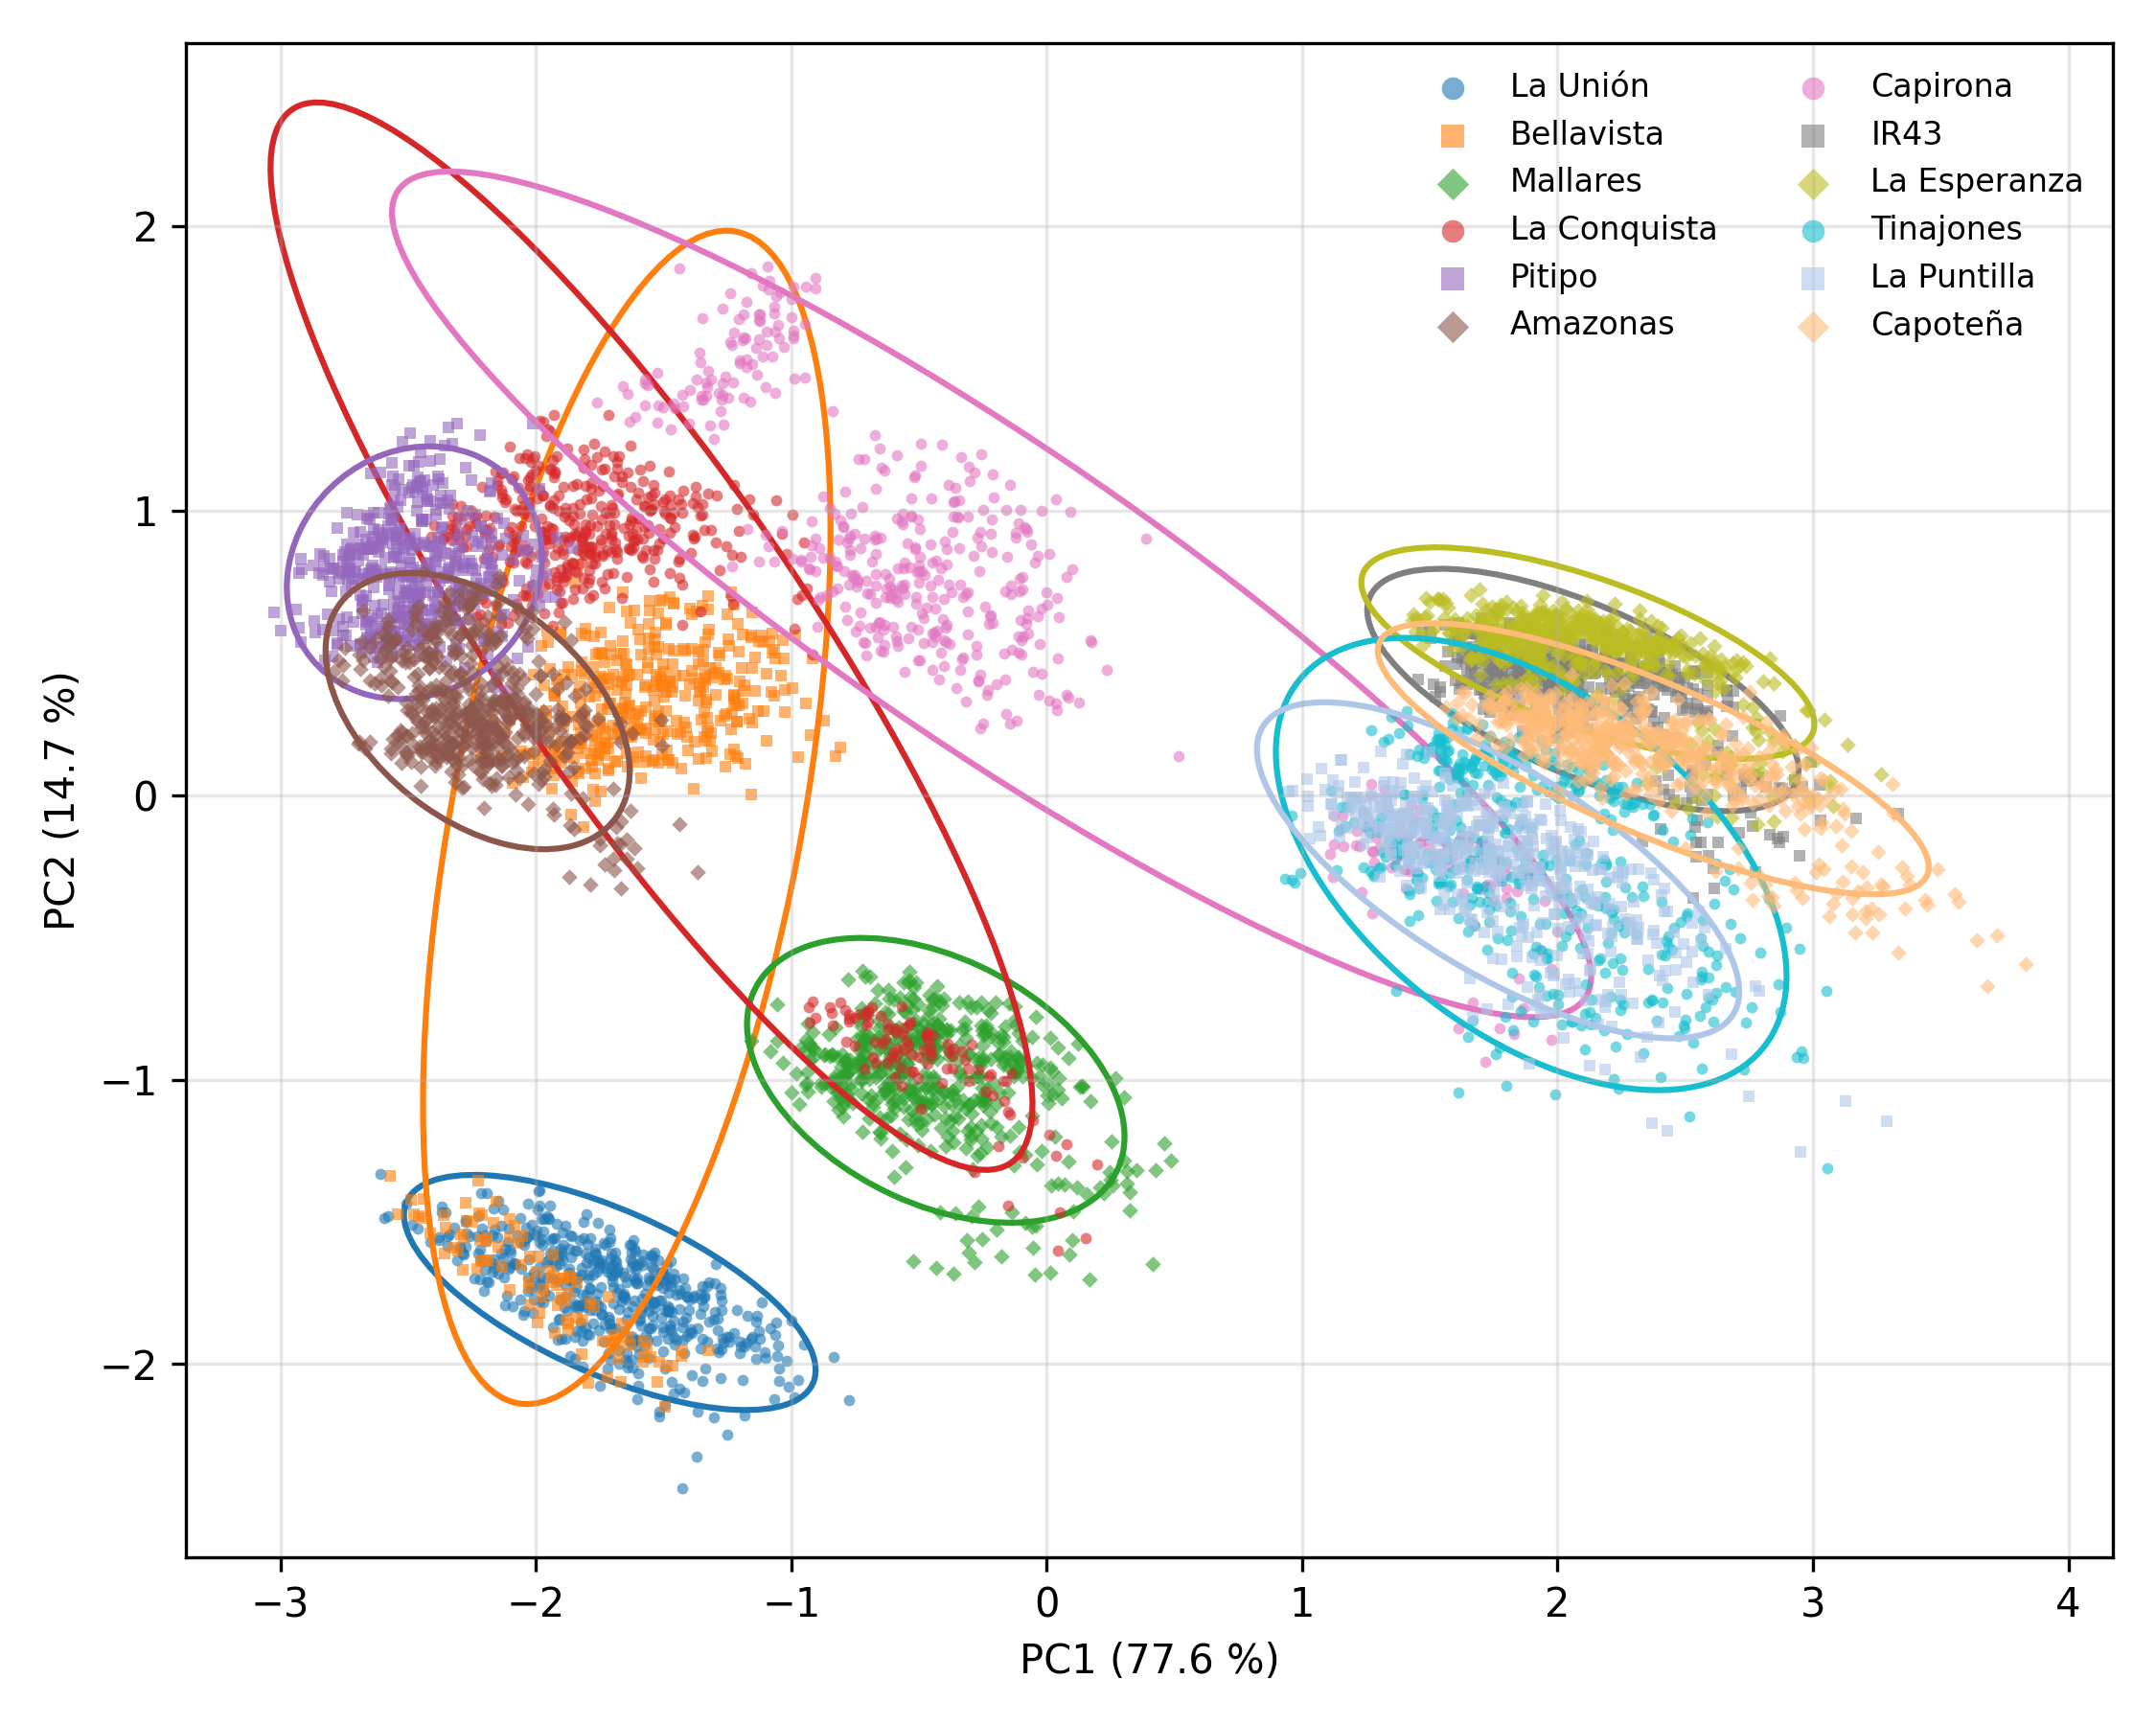
\includegraphics[width=\columnwidth]{Figures/fig_py_pca.png}
    \caption{Scores of the pre-treated profiles on the first two principal components (77.6\% and 14.7\% of the variance), one color and marker per variety, with 95\% confidence ellipses.}
    \label{fig_03}
\end{figure}

\added{Figure~\ref{fig_03} projects the spectra onto the first two principal components, with a 95\% confidence ellipse per variety. The first component separates two broad groups: seven varieties at negative scores (La Uni\'on, Bellavista, Mallares, La Conquista, Pitipo, Amazonas, Capirona) and five at positive scores (IR43, La Esperanza, Tinajones, La Puntilla, Capote\~na). Within the second group the second component partly separates IR43, La Esperanza and Capote\~na (upper) from Tinajones and La Puntilla (lower), with heavy overlap inside each pair. Within the first group, La Uni\'on forms a compact cloud at the bottom, Mallares a distinct cloud at the center, and Pitipo and Amazonas overlap at the upper left. Three varieties -- Bellavista, La Conquista and Capirona -- each appear as two separate clouds rather than one: part of Bellavista lies with La Uni\'on and part near Amazonas, part of La Conquista near Pitipo and part with Mallares, and Capirona in two lobes at the upper centre. This splitting is what stretches their ellipses across the plot; these three varieties are the ones with an image classified almost entirely as another variety (Section~\ref{sec_limitations}). The first two principal components therefore group the twelve varieties into three or four blocks rather than resolving them individually; PCA of FT-NIR spectra of rice has likewise shown groupings by variety and origin \citep{Tong2021}.}
\added{In the principal component analysis (263 bands), the first component alone carries 77.6\% of the total variance, the first two together 92.4\%, five components are needed to reach 99.4\%, and eleven for 99.9\%. The limited class separation visible here is therefore a two-dimensional cut through a signal that needs far more than two components to be summarized adequately, which is consistent with the classifiers using many discriminant or SVM dimensions rather than two.}

\subsection{Selected bands}

\begin{figure*}[htbp!]
    \centering
    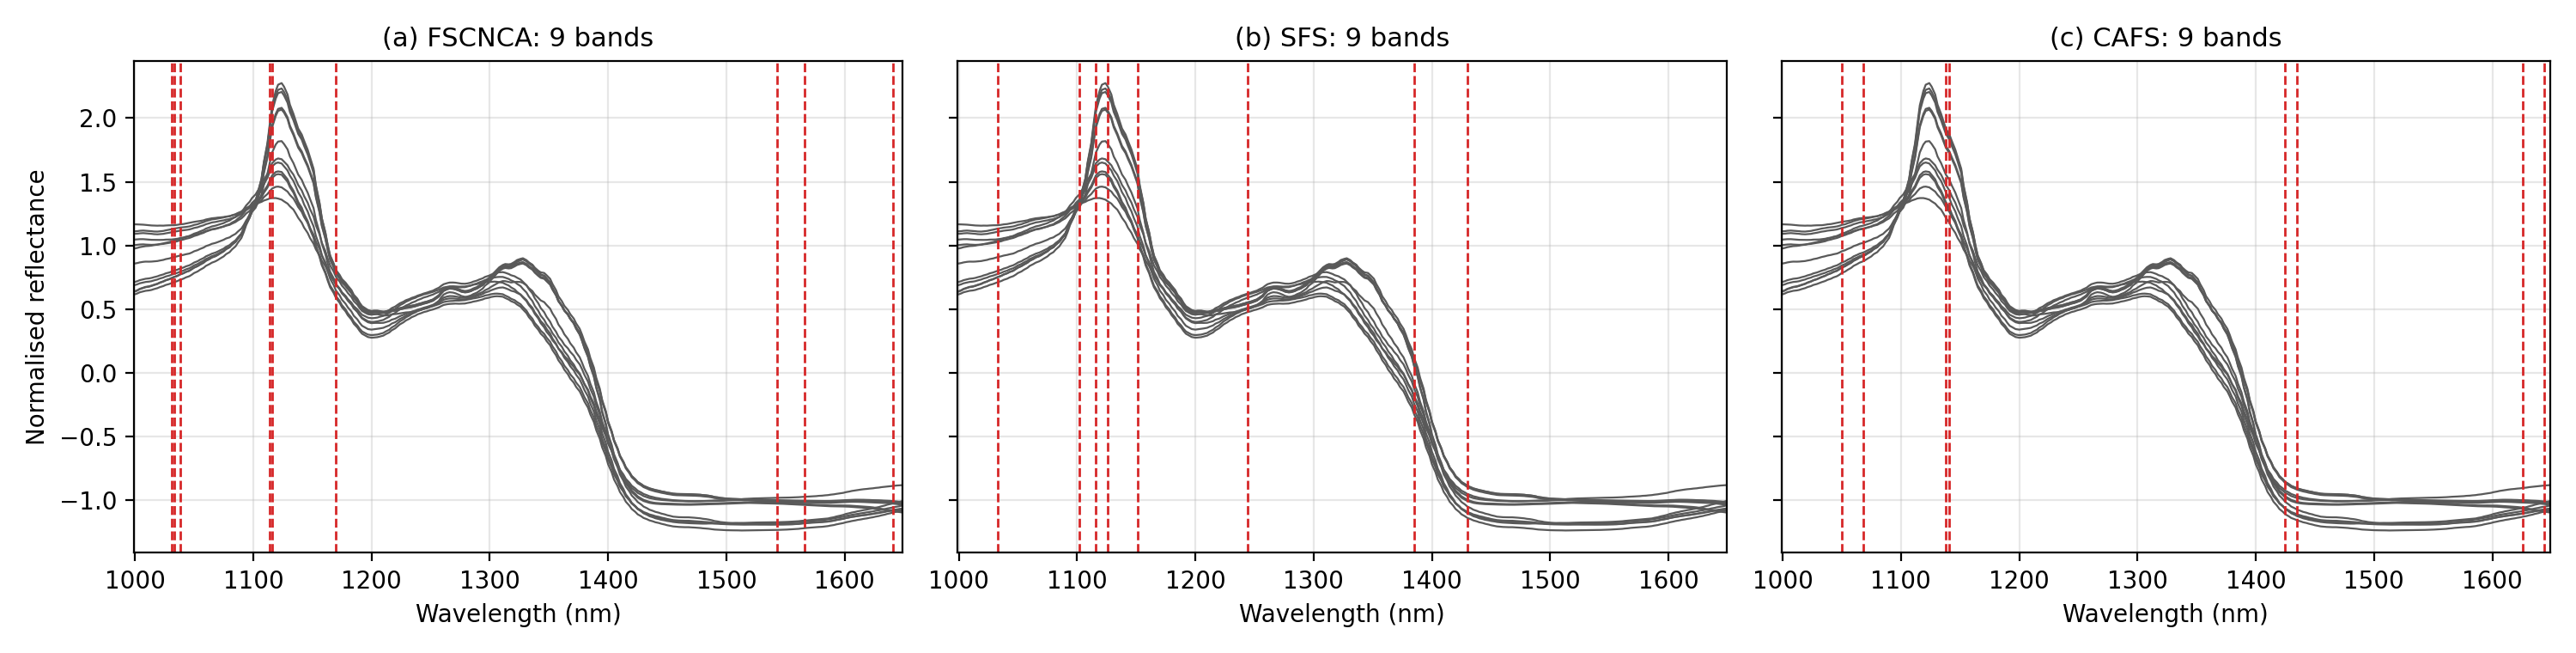
\includegraphics[width=\textwidth]{Figures/fig_py_bandas.png}
    \caption{Nine bands selected by (a) FSCNCA, (b) SFS and (c) CAFS, each fitted once on all 6000 profiles (red dashed lines), over the mean profiles of the twelve varieties. CAFS returned nine bands on its own.}
    \label{fig_04}
\end{figure*}

\added{Figure~\ref{fig_04} marks the bands selected by each method as vertical lines on the mean-profile background of Figure~\ref{fig_02}. FSCNCA: 1031, 1033, 1038, 1114, 1116, 1170, 1543, 1566 and 1641~nm. SFS: 1033, 1102, 1116, 1126, 1151, 1244, 1385, 1430 and 1649~nm. CAFS: 1050, 1068, 1138, 1141, 1425, 1435, 1626, 1644 and 1649~nm. All three methods place two to four bands on the rising edge and maximum between 1100 and 1150~nm, and one to three near the upper end of the range (1626--1649~nm). SFS and CAFS each place two bands in the fall into the O--H region (1385--1435~nm), where FSCNCA places none, choosing instead three bands near 1035~nm and two on the plateau at 1543--1566~nm. Only three wavelengths are shared exactly by two methods (1033 and 1116~nm by FSCNCA and SFS, 1649~nm by SFS and CAFS). That three reasonable methods agree so little on which bands matter, while reaching comparable accuracy (77--84\% with the SVM with one image per variety held out, Table~\ref{tab:sub9}), suggests that many bands are interchangeable; Section~\ref{sec_bands_results} tests this directly against randomly drawn subsets.}
The selected wavelengths should not be read as markers of individual compounds: NIR bands are broad, overlapping and highly correlated, so a selection points at regions whose combined C--H and O--H responses differ between varieties, not at constituents.


\subsection{Classification}\label{sec_classification}


\added{Table~\ref{tab:acc} gives the overall accuracy (Equation~\ref{eq_acc}) of the four classifiers on the full spectrum. Under the random division the SVM reaches 97.2\% and the ANN 97.1\%, which correspond to 99.53\% and 99.51\% in per-class one-vs-rest accuracy, and LDA and the L-SVM reach 90.4\% and 90.2\%. With one image per variety held out, accuracy falls to 87.8\% for the SVM, 88.2\% for the ANN, 86.7\% for LDA and 84.2\% for the L-SVM, and the standard deviation across splits grows from 0.5--0.8 to 6--7 points. The macro-averaged F1-score equals overall accuracy to within 0.1 points under the random division, but falls 1.8--2.2 points below it under the grouped division (SVM 85.9\%, ANN 86.4\%, LDA 84.7\%, L-SVM 82.0\%), because a held-out image misassigned as a whole lowers both the recall of its variety and the precision of the variety it is taken for. Compared over the 60 images (Section~\ref{sec_performance}; differences are means over images and can differ by 0.1--0.4 points from differences of the split means in Table~\ref{tab:acc}), the drop from random to grouped division is significant for all four classifiers (adjusted $p<10^{-4}$): 9.4 points for the SVM (95\% confidence interval 4.3--15.5), 9.0 for the ANN (4.2--15.0), 6.1 for the L-SVM (3.1--9.9) and 3.8 for LDA (1.7--6.2). Under the random division the SVM exceeds LDA and the L-SVM by 6.8 and 6.9 points (intervals 3.0--11.7 and 3.2--11.6; $p\le0.0003$); the lead of the ANN over them is as large (6.7--6.8 points) but less consistent across images ($p=0.067$), the SVM and the ANN differ by only 0.1 points (consistently across images, $p=0.011$, but negligibly), and LDA and the L-SVM do not differ ($p=1.0$). With one image held out, the SVM, the ANN and LDA no longer differ (differences of 0.2--1.4 points, with intervals that include zero), and only the lead of the SVM over the L-SVM remains (3.7 points, interval 1.4--6.3, $p=0.023$).}

\begin{table*}[htbp!]
    \centering
    \caption{Overall accuracy and macro-averaged F1-score (\%, mean $\pm$ SD over 30 splits: six repetitions of a five-fold cross-validation) of the four classifiers on the full spectrum, with grains divided at random and with one image per variety held out. L-SVM: linear SVM on unstandardized bands (Section~\ref{sec_building}). Last column: the per-class one-vs-rest (OvR) accuracy of the SVM, for comparison with studies that report it.}
    \label{tab:acc}
    \begin{tabular}{lccccc}
    \hline
    Division, metric & SVM & L-SVM & LDA & ANN & SVM, OvR \\
    \hline
    Random, accuracy             & 97.2 $\pm$ 0.5 & 90.2 $\pm$ 0.7 & 90.4 $\pm$ 0.8 & 97.1 $\pm$ 0.5 & 99.5 $\pm$ 0.1 \\
    Random, macro-F1             & 97.2 $\pm$ 0.5 & 90.2 $\pm$ 0.7 & 90.4 $\pm$ 0.8 & 97.1 $\pm$ 0.5 & -- \\
    One image held out, accuracy & 87.8 $\pm$ 6.3 & 84.2 $\pm$ 7.0 & 86.7 $\pm$ 6.7 & 88.2 $\pm$ 6.5 & 98.0 $\pm$ 1.1 \\
    One image held out, macro-F1 & 85.9 $\pm$ 8.0 & 82.0 $\pm$ 8.8 & 84.7 $\pm$ 8.4 & 86.4 $\pm$ 8.2 & -- \\
    \hline
    \end{tabular}
\end{table*}

\added{Figure~\ref{fig:cm} shows the confusion matrices, pooled over the 30 splits. The errors concentrate in a few pairs of varieties: with the SVM and the ANN under the random division, IR43 and La Esperanza are taken for each other in 7--8\% of cases, La Conquista for Mallares in 2--5\%, Tinajones and La Puntilla in 3--5\% and Pitipo and Amazonas in 1--2\%, and LDA and the L-SVM confuse the same pairs at about twice these rates (IR43 and La Esperanza 14--18\%). Other confusions involve whole images. Under the random division LDA and the L-SVM already assign about 20\% of Bellavista to La Uni\'on and 20\% of La Conquista to Mallares -- one image in each case -- whereas the SVM and the ANN, trained on other grains of the same images, do so for only 1--5\%; with the images held out, all four classifiers lose them, and Capirona is taken for La Puntilla in 14--20\% of cases, again one image (Section~\ref{sec_limitations}). This is the mechanism behind most of the lead of the SVM and the ANN under the random division.}

\begin{figure*}[htbp!]
    \centering
    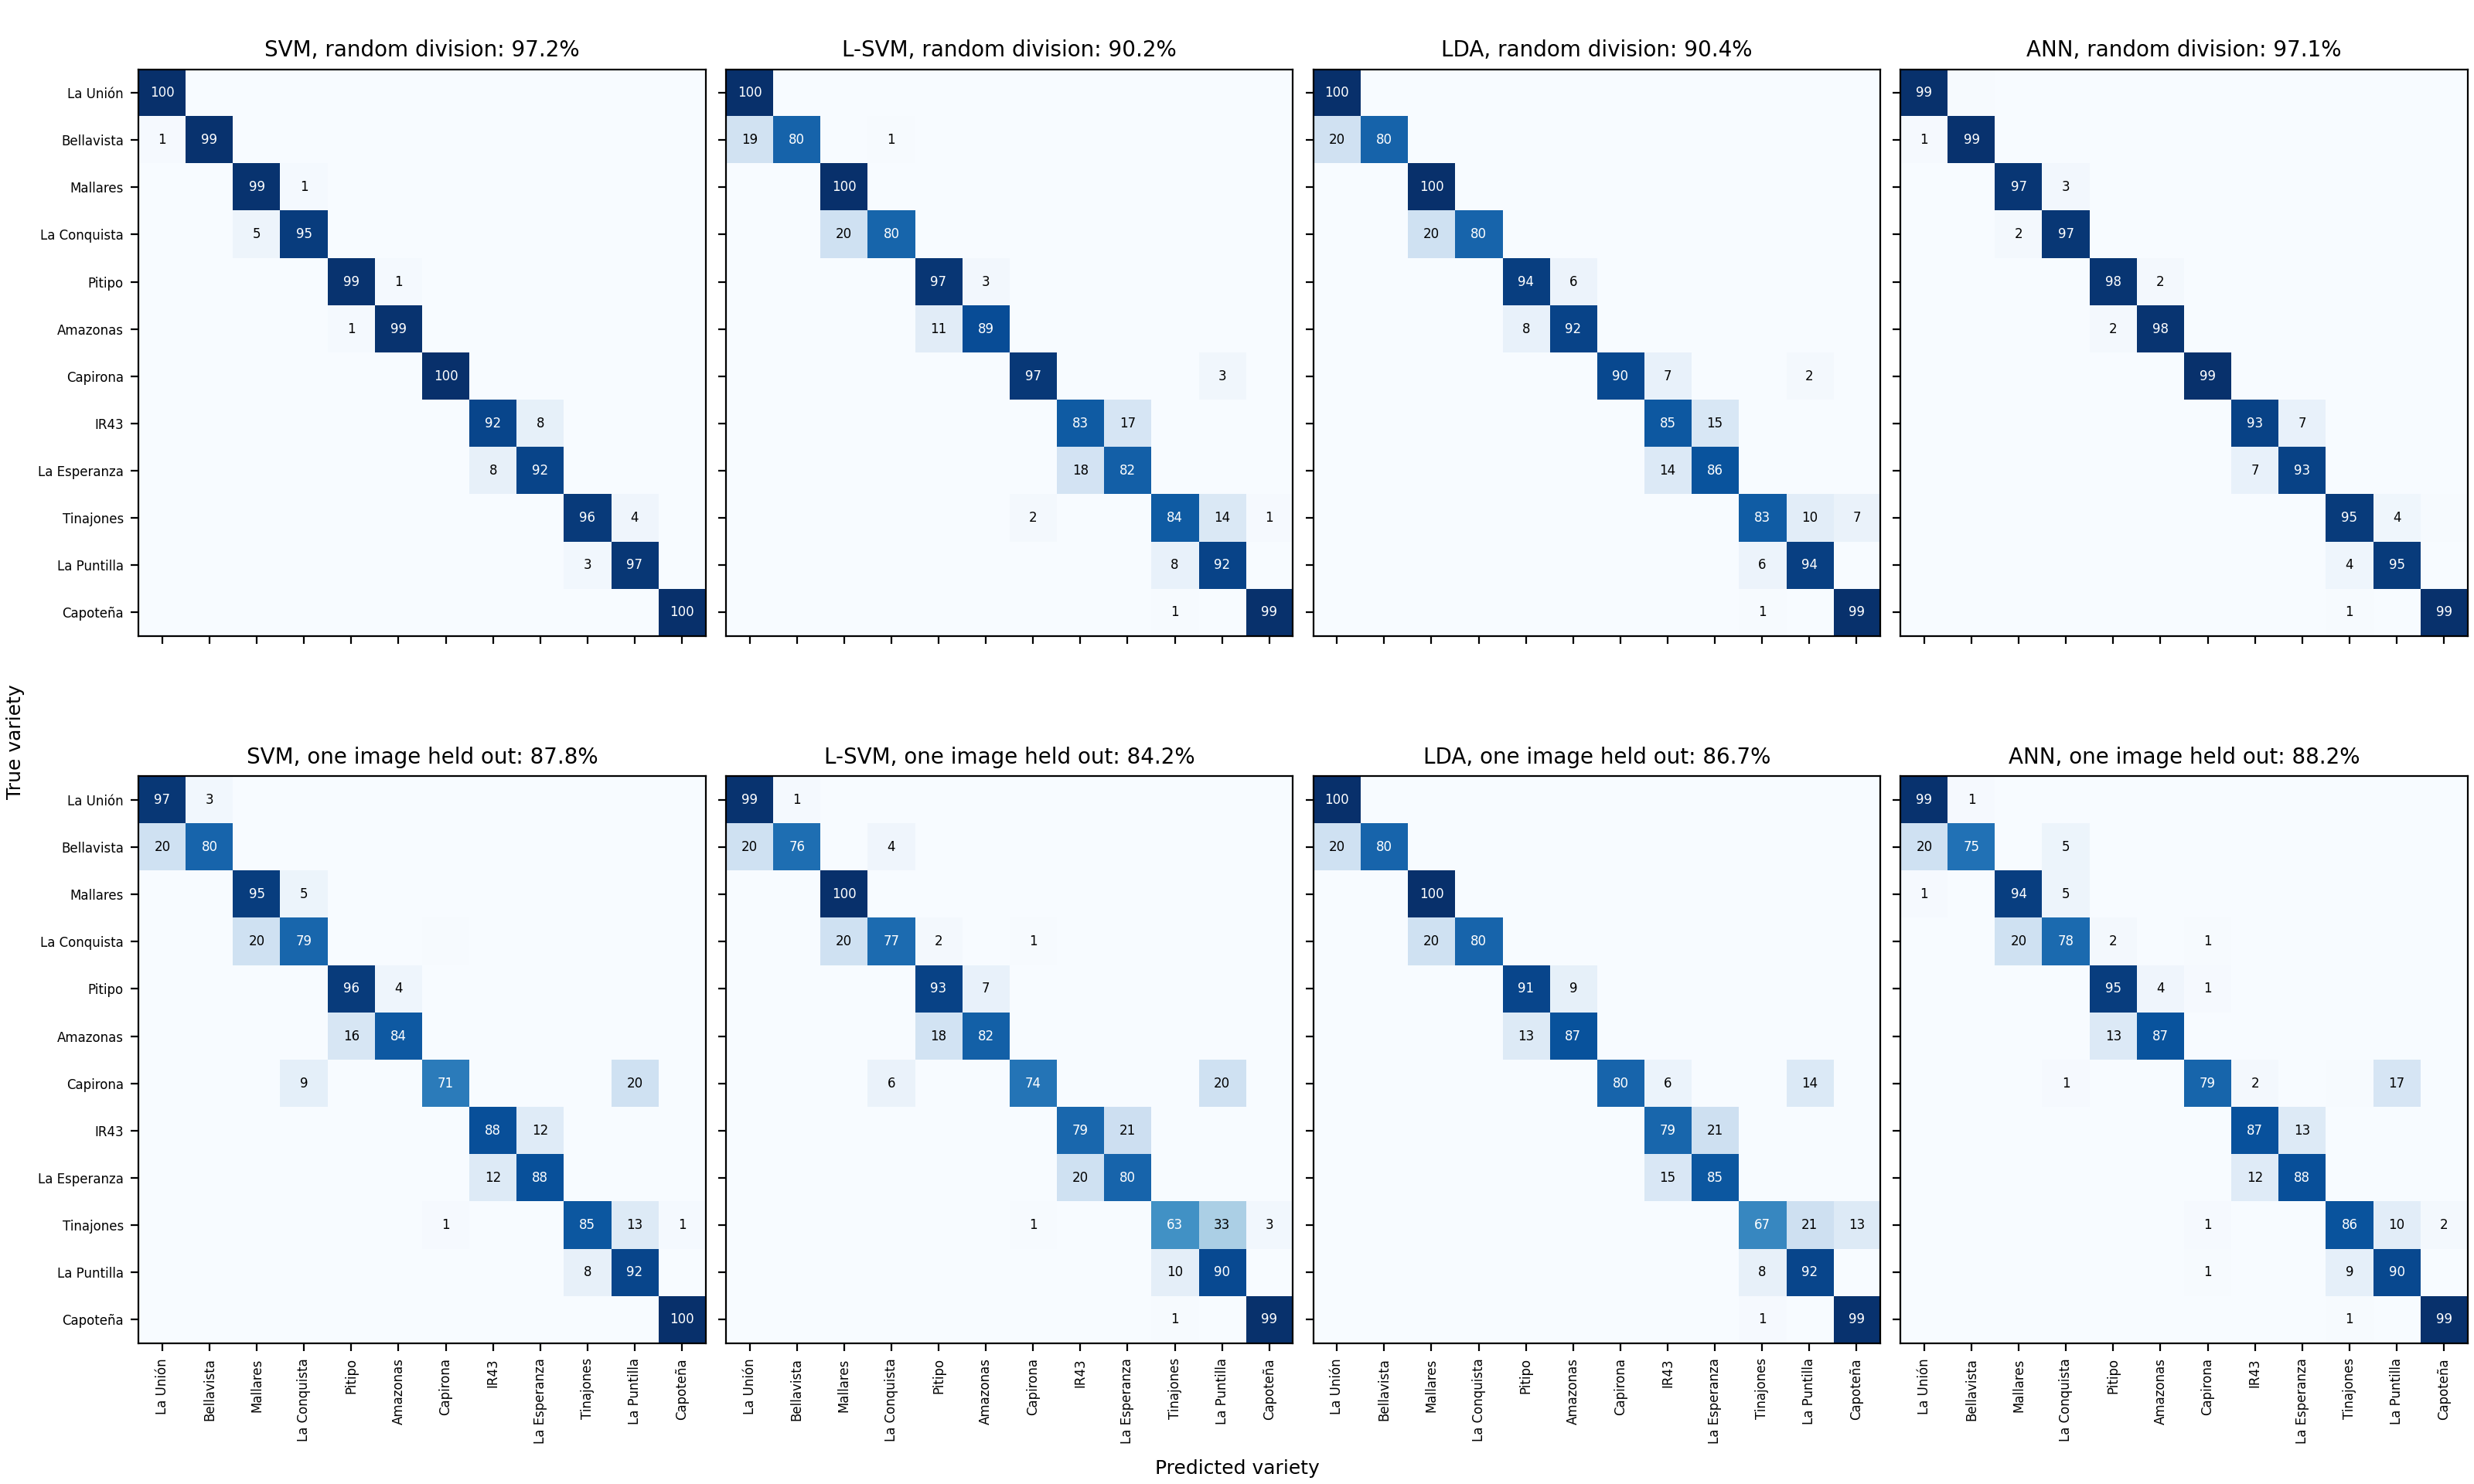
\includegraphics[width=\textwidth]{Figures/fig_unf_cm.png}
    \caption{\added{Confusion matrices (percent of the grains of each true variety, pooled over the 30 splits) of the four classifiers on the full spectrum: random division (top) and one image per variety held out (bottom). Panel titles give overall accuracy. Values below 0.5\% are not shown.}}
    \label{fig:cm}
\end{figure*}


\subsection{Random-subset baseline for band selection}\label{sec_bands_results}

\added{The nine-band subsets obtained by applying each method once to all 6000 spectra (Figure~\ref{fig_04}) were tested directly against random nine-band subsets with one image per variety held out (Table~\ref{tab:sub9}). The SFS subset beats the random mean with the three linear classifiers, by 3.6--7.3 points, and outperforms 86--99\% of the random subsets, but not with the ANN (+0.1 points), whose hidden layer has only three units with nine bands. The FSCNCA subset is ahead of the random mean by 1.3--3.8 points with the linear classifiers and 7.1 points behind it with the ANN. The CAFS subset is ahead with the L-SVM (3.2 points) but behind with the SVM and LDA (3.3 and 2.4 points). All differences except those of SFS and CAFS with the ANN are consistent across splits (Holm-adjusted $p\le0.004$). These subsets were selected with all the spectra, so part of their advantage may come from the test grains taking part in the selection: when selection is fitted on the training part of each split, as above, FSCNCA no longer beats random subsets and SFS does so mainly with 5--10 bands.}
\added{Each selection method was compared against randomly drawn band subsets of the same size under the grouped division, since an advantage from selecting bands only matters if it survives on grains from a new image (protocol in Section~\ref{sec_feature_selection}). CAFS (a covering array of 12 rows for 263 bands in the first iteration) shrank the set from 263 to about 137, 80, 39, 24, 16 and 14 bands and returned the best-scoring subset over all iterations (7--25 bands); the subset of each iteration and the returned subset were compared against random subsets of the same size. Differences below are paired over splits and computed from unrounded values, so they can differ by 0.1 from differences of the rounded table entries.}
\added{Tables~\ref{tab:bands_unf} and \ref{tab:bands_cafs} and Figure~\ref{fig:bands_unf} summarize the results. SFS is at or above the random mean at every $k$, by 6--9 points at $k=5$ and by at most 0.6 points at $k=40$. FSCNCA is never clearly better than random: 1.5--2.6 points ahead at $k\le10$, within 0.5 points of random at $k=20$ and up to 1.4 points below it at $k=40$. CAFS falls 1.0--3.0 points below the random mean at every iteration shown, and the subset it returns -- 19 bands on average, from 7 to 25 depending on the split -- is also below random (80.1\% against 82.4\% with the SVM, 79.2\% against 82.2\% with LDA). For every method, size and classifier, the selected subset lies within the 5--95\% range of the random subsets. The advantage of selecting bands over drawing them at random is therefore at most modest, largest for SFS with very few bands, and vanishes as more bands are kept. Paired over the splits with Holm adjustment across the 30 comparisons, the paired $t$-test finds SFS better than random at 5 bands (by 6.2 points with the SVM and 8.8 with LDA; adjusted $p=0.002$ for both), at 10 bands (3.6 and 6.0 points; $p=0.007$ and $0.0007$) and at 20 bands with LDA only (2.3 points; $p=0.0005$); FSCNCA never better, and worse at 40 bands with the SVM (1.4 points, $p=0.010$); and CAFS never better, but worse than random at iterations 1--4 with the SVM (by 1.6--2.2 points, adjusted $p\le0.02$) and at iterations 2 and 3 with LDA (2.4 and 2.7 points, adjusted $p=0.042$ and $0.006$); its returned subset is not significantly different from random ($p=0.18$ with the SVM, $0.56$ with LDA), although it lies 2.3 and 3.0 points below the random mean. With 10 splits the Wilcoxon signed-rank test cannot reach an adjusted $p<0.05$ for any of the 30 comparisons (its smallest attainable unadjusted $p$ is 0.002), so these differences rest on the $t$-test alone, and the splits share images, so they are not independent.}

\begin{table*}[htbp!]
    \centering
    \caption{\added{Overall accuracy (\%, mean $\pm$ SD over the 30 splits, one image per variety held out) of the nine-band subsets obtained by applying each selection method once to all the spectra (Figure~\ref{fig_04}), against 30 random nine-band subsets per split (mean, and 5--95\% range over all 900 random draws). Fraction: share of random subsets outperformed, averaged over splits. The subsets were selected with all the spectra, which favors them. With nine bands the ANN has three hidden units.}}
    \label{tab:sub9}
    \begin{tabular}{llcccc}
    \hline
    Classifier & Subset & Accuracy & Random mean (5--95\%) & Difference & Fraction \\
    \hline
    SVM   & FSCNCA & 81.9 $\pm$ 7.7 & 80.6 (68.7--91.3) & $+$1.3 & 0.61 \\
          & SFS    & 84.2 $\pm$ 7.2 & 80.6 (68.7--91.3) & $+$3.6 & 0.86 \\
          & CAFS   & 77.3 $\pm$ 6.7 & 80.6 (68.7--91.3) & $-$3.3 & 0.16 \\
    L-SVM & FSCNCA & 72.8 $\pm$ 7.8 & 69.0 (55.4--80.0) & $+$3.8 & 0.77 \\
          & SFS    & 76.2 $\pm$ 7.1 & 69.0 (55.4--80.0) & $+$7.3 & 0.99 \\
          & CAFS   & 72.1 $\pm$ 6.9 & 69.0 (55.4--80.0) & $+$3.2 & 0.72 \\
    LDA   & FSCNCA & 80.2 $\pm$ 7.5 & 78.5 (64.7--89.8) & $+$1.8 & 0.67 \\
          & SFS    & 85.1 $\pm$ 7.3 & 78.5 (64.7--89.8) & $+$6.6 & 0.98 \\
          & CAFS   & 76.1 $\pm$ 7.1 & 78.5 (64.7--89.8) & $-$2.4 & 0.28 \\
    ANN   & FSCNCA & 64.2 $\pm$ 7.4 & 71.3 (56.4--84.4) & $-$7.1 & 0.23 \\
          & SFS    & 71.4 $\pm$ 8.8 & 71.3 (56.4--84.4) & $+$0.1 & 0.49 \\
          & CAFS   & 72.1 $\pm$ 7.0 & 71.3 (56.4--84.4) & $+$0.8 & 0.51 \\
    \hline
    \end{tabular}
\end{table*}



\begin{table*}[htbp!]
    \centering
    \caption{\added{Overall accuracy (\%, mean $\pm$ SD) of SFS- and FSCNCA-selected bands against 30 randomly drawn subsets of the same size, with one image per variety held out (10 splits; same splits and random subsets for both methods). The SD of the random subsets is over 300 evaluations (30 subsets in each of 10 splits), that of SFS and FSCNCA over the 10 splits.}}
    \label{tab:bands_unf}
    \resizebox{0.75\textwidth}{!}{
    \begin{tabular}{rcccccc}
    \hline
    \multirow{2}{*}{Bands $k$} & \multicolumn{3}{c}{SVM} & \multicolumn{3}{c}{LDA} \\
     & SFS & FSCNCA & Random & SFS & FSCNCA & Random \\
    \hline
    5  & 80.2 $\pm$ 5.6 & 76.1 $\pm$ 6.8 & 74.0 $\pm$ 7.4 & 79.8 $\pm$ 3.9 & 73.6 $\pm$ 7.7 & 71.0 $\pm$ 6.3 \\
    10 & 84.2 $\pm$ 6.7 & 82.1 $\pm$ 5.6 & 80.6 $\pm$ 6.7 & 85.0 $\pm$ 4.4 & 81.4 $\pm$ 4.2 & 79.0 $\pm$ 5.2 \\
    20 & 85.5 $\pm$ 5.8 & 83.1 $\pm$ 6.0 & 83.6 $\pm$ 6.2 & 86.2 $\pm$ 4.2 & 84.2 $\pm$ 4.8 & 83.8 $\pm$ 4.5 \\
    40 & 85.3 $\pm$ 6.3 & 83.9 $\pm$ 6.4 & 85.3 $\pm$ 6.1 & 86.5 $\pm$ 4.5 & 85.4 $\pm$ 5.2 & 85.9 $\pm$ 4.8 \\
    \hline
    \end{tabular}
    }
    
    
\end{table*}

\begin{table*}[htbp!]
    \centering
    \caption{\added{Overall accuracy (\%, mean $\pm$ SD over splits) of CAFS-selected bands against 30 randomly drawn subsets of the same size, with one image per variety held out (10 splits). CAFS (settings of Section~\ref{sec_feature_selection}) sets its own subset size, so sizes are means over the splits that reached each iteration; iterations 7--9, reached by 5, 2 and 1 of the 10 splits, are not shown. Last row: the subset CAFS returns, the best-scoring over all iterations.}}
    \label{tab:bands_cafs}
    \begin{tabular}{rccccc}
    \hline
    \multirow{2}{*}{Bands (mean)} & \multirow{2}{*}{Splits} & \multicolumn{2}{c}{SVM} & \multicolumn{2}{c}{LDA} \\
     & & CAFS & Random & CAFS & Random \\
    \hline
    137 & 10 & 85.0 $\pm$ 6.5 & 86.7 $\pm$ 6.2 & 85.5 $\pm$ 5.6 & 86.5 $\pm$ 4.9 \\
    80  & 10 & 84.1 $\pm$ 6.8 & 86.2 $\pm$ 6.1 & 84.1 $\pm$ 5.4 & 86.5 $\pm$ 4.8 \\
    39  & 10 & 83.3 $\pm$ 6.5 & 85.2 $\pm$ 6.1 & 83.2 $\pm$ 5.1 & 85.9 $\pm$ 4.6 \\
    24  & 10 & 81.9 $\pm$ 6.5 & 84.1 $\pm$ 6.0 & 82.0 $\pm$ 5.8 & 84.6 $\pm$ 4.5 \\
    16  & 10 & 79.4 $\pm$ 6.8 & 82.4 $\pm$ 5.8 & 79.9 $\pm$ 7.0 & 82.4 $\pm$ 4.7 \\
    14  & 10 & 78.4 $\pm$ 6.3 & 80.9 $\pm$ 5.7 & 78.0 $\pm$ 6.1 & 80.4 $\pm$ 5.7 \\
    \hline
    Returned, 19 (7--25) & 10 & 80.1 $\pm$ 6.6 & 82.4 $\pm$ 5.7 & 79.2 $\pm$ 5.8 & 82.2 $\pm$ 5.2 \\
    \hline
    \end{tabular}
\end{table*}

\begin{figure*}[htbp!]
    \centering
    \subfloat[SFS]{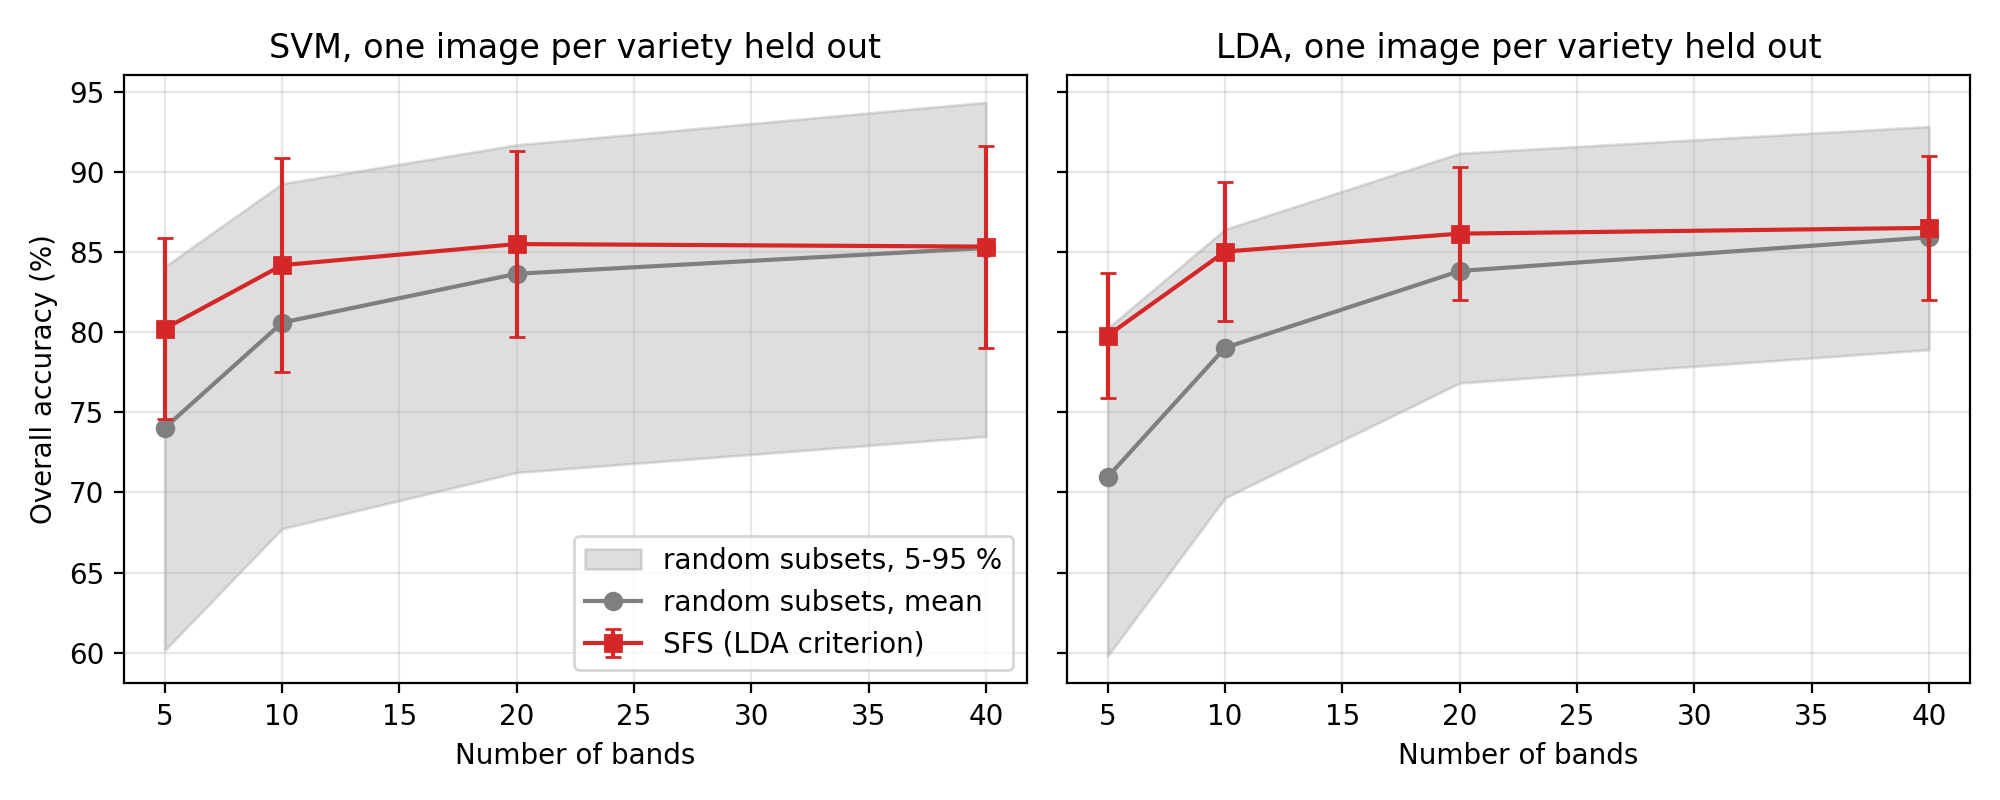
\includegraphics[width=0.49\textwidth]{Figures/fig_unf_bandas.png}}
    \hfill
    \subfloat[FSCNCA]{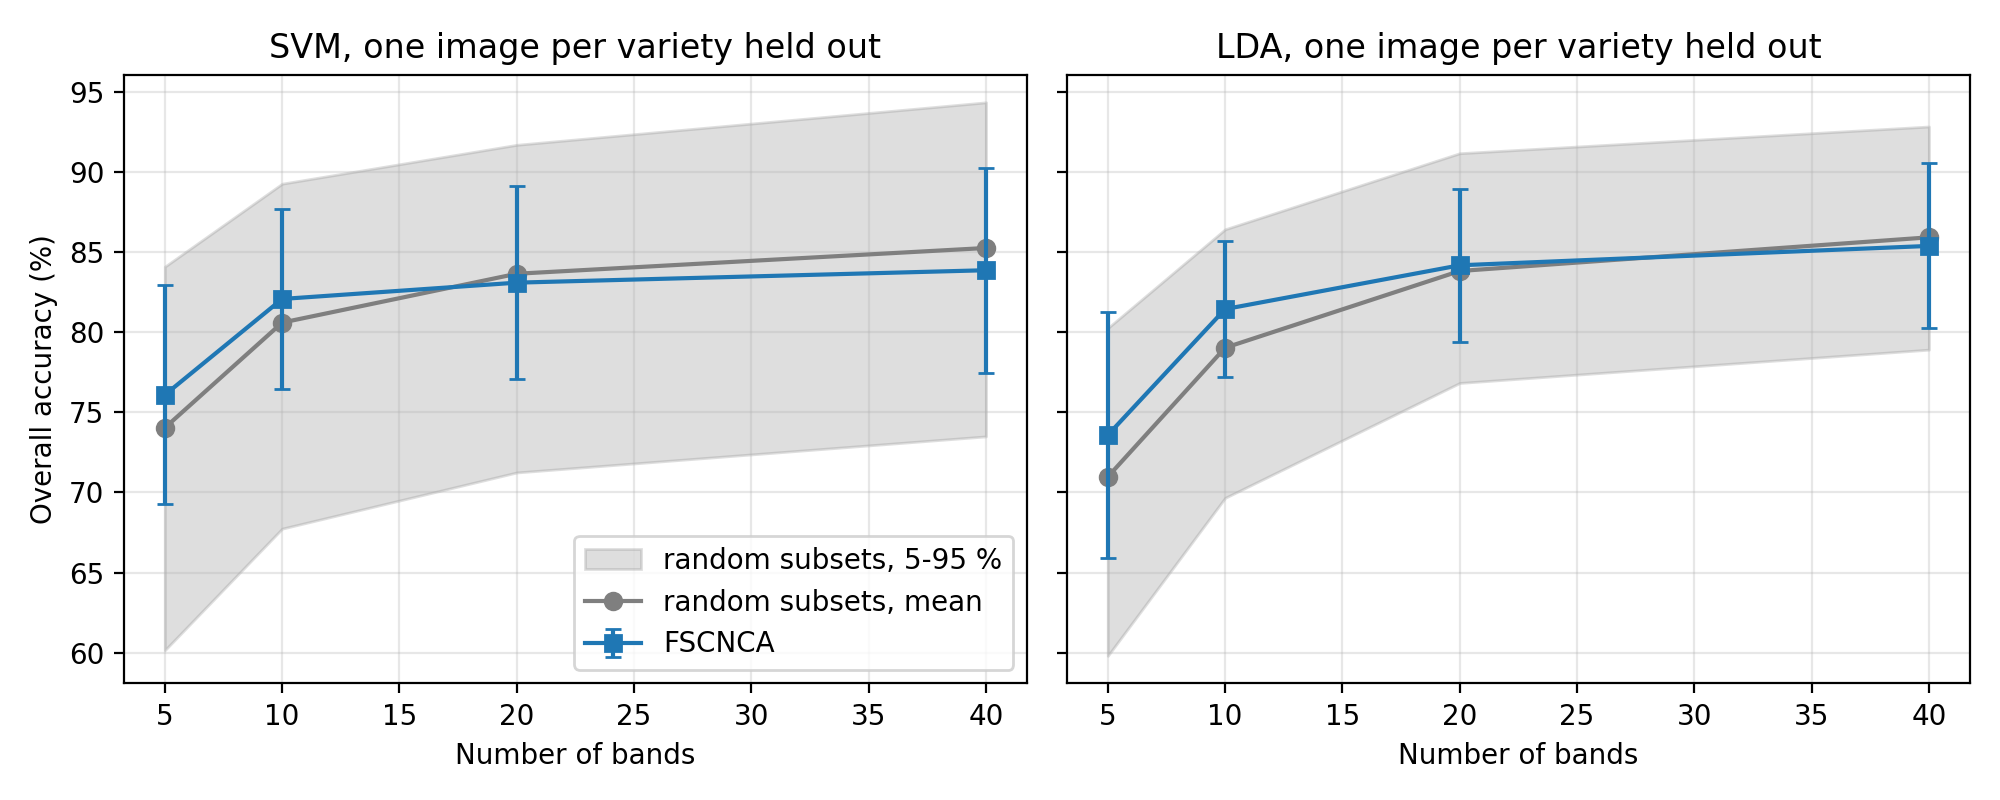
\includegraphics[width=0.49\textwidth]{Figures/fig_unf_bandas_fscnca.png}}\\
    \subfloat[CAFS]{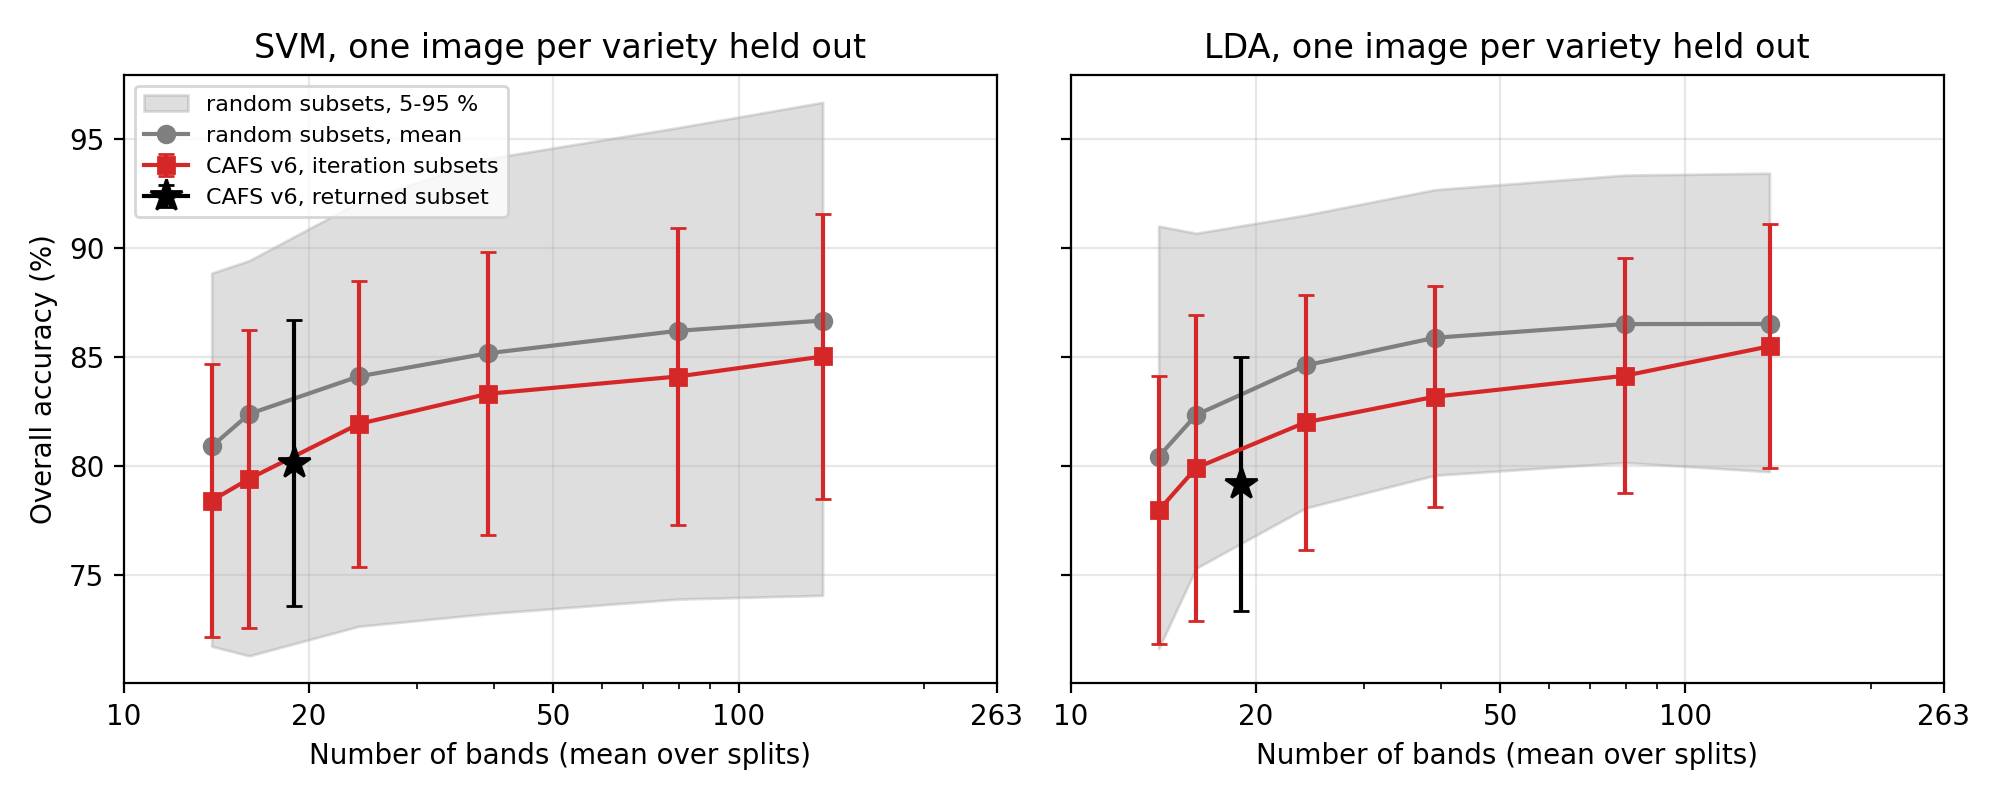
\includegraphics[width=0.49\textwidth]{Figures/fig_unf_bandas_cafs_v6.png}}
    \caption{Overall accuracy of band subsets selected by (a) SFS, (b) FSCNCA and (c) CAFS (colored), against 30 randomly drawn subsets of the same size (gray line: mean; gray band: 5--95\% range), with one image per variety held out, for SVM (left) and LDA (right). In (c) the horizontal axis is logarithmic and gives the mean subset size per CAFS iteration (iterations 1--6, reached by all 10 splits); the star is the subset CAFS returns.}
    \label{fig:bands_unf}
\end{figure*}




\added{\section{Discussion}\label{sec_discussion}

\subsection{Validation design and metric}
The accuracies obtained under random and grouped division estimate different quantities. Under the random division the test grains come from images also represented in training; under the grouped division they come from another image of the same lot, which is closer to how an instrument would be used, though still optimistic for a new lot, season or session. The gap between them, about 9 points for the SVM, depends on how much grains imaged together share, a property of the acquisition rather than of the classifier, so it cannot be carried to another data set as a correction. The same distinction bears on the choice of classifier: the 7-point lead of the SVM and the ANN over LDA and the L-SVM under the random division disappears against LDA under the grouped division, where the SVM, the ANN and LDA no longer differ, and shrinks to 3.7 points against the L-SVM. The per-class one-vs-rest accuracy, in turn, compresses differences by a factor of six for twelve classes and cannot fall below 83.3\%. The studies in Table~\ref{Table1} report best accuracies of 95--100\%; where a study does not state whether grains from one image or session were kept together, or which accuracy it reports, its figures and ours cannot be compared as they stand.

\subsection{Band selection}
The three selection methods retained different bands (Figure~\ref{fig_04}). Nine-band subsets selected once with all the spectra beat random nine-band subsets clearly only for SFS with the linear classifiers; FSCNCA led by a few points at most and CAFS was above or below random depending on the classifier (Table~\ref{tab:sub9}); because they were chosen with all the spectra, the training-only analysis is the fairer test. Fitted on training data only and tested on held-out images, SFS beat randomly drawn subsets of the same size at 5 and 10 bands, by about 4--9 points -- the range that matters for an instrument with few channels -- and at 20 bands with LDA, but not at 40; FSCNCA led random subsets by at most 2.6 points at 5--10 bands and by no more than 0.4 points from 20 bands on; and CAFS trailed them by 1.0--3.0 points at every size. Neighboring NIR bands are highly correlated, so many subsets of adequate size perform similarly. A band-selection result on spectra of this kind should therefore be reported against a random-subset control of the same size.

\subsection{Chemical interpretation}
Relative to grain-to-grain scatter, the mean profiles differ most on the falling edge between 1100 and 1150~nm, which covers the C--H band assigned to starch in rice flour \citep{Shao2011starch} and leads into the C--H second-overtone minimum near 1200~nm shared by starch and lipid, and on the fall into the O--H absorption of water between 1340 and 1430~nm (Section~\ref{sec_mean_profiles}). These differences are consistent with differences in starch structure, lipid and moisture between varieties, but this paper does not test that attribution, which would require composition measured on the same grains that were imaged.

\subsection{Limitations}\label{sec_limitations}
Each variety is a single lot imaged in one session, so variety is confounded with lot and acquisition time. The confused pairs (IR43 and La Esperanza, Tinajones and La Puntilla, Pitipo and Amazonas, La Conquista and Mallares) are adjacent in the list of Section~2.1, which follows the order in which the varieties were coded and, we assume, imaged; if so, slow drift of the instrument would contribute to the similarity of neighboring varieties. Three of the 60 images -- image~5 of Bellavista, image~1 of La Conquista and image~5 of Capirona -- are classified almost entirely as La Uni\'on, Mallares and La Puntilla when held out, although their labels are confirmed; within a single lot and session, the conditions of one image can thus outweigh the differences between varieties. In the within-training selection, the internal cross-validation of SFS and CAFS groups blocks of 10 rows rather than whole images, so grains of one image can sit on both sides of the internal criterion, which may reward bands specific to an acquisition. They are the extreme cases of a wider image effect: three more images (image~1 of Amazonas, image~1 of La Esperanza and image~3 of Tinajones) have fewer than two thirds of their grains classified correctly by every classifier. Finally, the grouping into images of 100 grains follows the acquisition protocol and has not been checked against image identifiers.}

\section{Conclusion}

\added{Twelve Peruvian rice varieties were discriminated from NIR-HSI spectra of single grains with an overall accuracy of about 97\% for the linear SVM and the ANN when grains were divided at random and about 88\% when whole images were held out; LDA reached 90\% and 87\%, and the L-SVM 90\% and 84\%. The per-class one-vs-rest accuracy would show 99.5\% and 98.0\% for the SVM and hide most of this drop. With images held out, the SVM, the ANN and LDA did not differ, and only the 3.7-point lead of the SVM over the L-SVM remained. Band selection reduced the number of bands without consistently identifying better ones: fitted on training data only, only SFS beat randomly drawn subsets of the same size, and mainly with 5--10 bands; nine-band subsets selected once with all the spectra did better for SFS, but the test grains took part in choosing them. These estimates assume that each block of 100 consecutive grains is one image. Reporting overall accuracy, validating on images not used for training, and benchmarking band selection against random subsets would make accuracies comparable between studies.}



% ================================================================================================
\section*{CRediT authorship contribution statement}

\begin{table*}[htbp!]
    \centering
    \begin{tabular}{lcccccccccccccc}
    \hline
    Author & CON & DAT & FOR & FUN & INV & MET & PRO & RES & SOF & SUP & VAL & VIS & WOD & WRE \\
    \hline
    Himer Avila-George &  &  &  &  &  &  &  &  &  &  &  &  &  &  \\
    Nicole Briceño &  &  &  &  &  &  &  &  &  &  &  &  &  &  \\
    Cecilia Risco &  &  &  &  &  &  &  &  &  &  &  &  &  &  \\
    Tony Chuquizuta &  &  &  &  &  &  &  &  &  &  &  &  &  &  \\
    Aldo F. Combariza & \checkmark & \checkmark & \checkmark &  &  & \checkmark &  & \checkmark & \checkmark &  & \checkmark & \checkmark & \checkmark & \checkmark \\
    Wilson Castro & \checkmark & \checkmark & \checkmark & \checkmark & \checkmark & \checkmark & \checkmark & \checkmark & \checkmark & \checkmark & \checkmark & \checkmark & \checkmark & \checkmark \\
    \hline
    \end{tabular}
    \caption{CRediT authorship contributions. CON, Conceptualization; DAT, Data curation; FOR, Formal analysis; FUN, Funding acquisition; INV, Investigation; MET, Methodology; PRO, Project administration; RES, Resources; SOF, Software; SUP, Supervision; VAL, Validation; VIS, Visualization; WOD, Writing -- original draft; WRE, Writing -- review \& editing.}
    \label{tab:credit}
\end{table*}

The contributions of each author are given in Table~\ref{tab:credit}.

\section*{Declaration of competing interest}
The authors declare that they have no known competing financial interests or personal relationships that could have appeared to influence the work reported in this paper.

\section*{Funding}
This work was supported by [PENDIENTE: funder, programme and grant number] (W. Castro). [PENDIENTE: funding of the other authors, if any.] A.F. Combariza received no specific funding for this work.

\section*{Data availability}
The pre-treated spectral matrix, the class labels, all analysis code and the intermediate results are available at \texttt{https://github.com/\allowbreak In-Silico-RG/\allowbreak Arroz\_NIR\_Replication}.

\section*{Declaration of generative AI and AI-assisted technologies in the writing process}
During the preparation of this work the authors used Claude Code (Anthropic) to write and run the analysis code and statistics and to draft parts of the text. After using this tool, the authors reviewed and edited the content as needed and take full responsibility for the content of the published article.

%% BIBLIOGRAPHY
% ================================================================================================
\bibliographystyle{elsarticle-num-names}
\bibliography{references2}

\end{document}
